\chapter{Ergebnisse}
\label{ch:ergebnisse}

Im folgenden Kapitel werden die Ergebnisse der energetischen Simulation, der Exergieanalyse und der wirtschaftlichen Bewertung dokumentiert. Dabei werden die zentralen Kennzahlen des Einkolonnen- und Doppelkolonnenprozesses gegenübergestellt. Für die wirtschaftliche Auswertung werden zusätzlich die kleine und große Anlagenvariante betrachtet.

\section{Ergebnisse der energetischen Prozesssimulation}
\label{sec:ergebinnse_simulation}

Die Ergebnisse der Hauptströme der beiden modellierten Prozesse sind in Tabelle \ref{tab:stream_comparison_compact} zusammengefasst. Bei den dort aufgeführten Verlustströmen handelt es sich um die sauerstoffangereicherten Sumpfströme aus den Kolonnen. Dabei zeigt sich, dass alle im Kapitel \ref{ch:prozess} definierten Zielvorgaben hinsichtlich der geforderten Produktmenge und Reinheit vollständig eingehalten wurden. Alle hier betrachteten Edukt- und Produktströme liegen im gasförmigen Zustand vor. \\
Hinsichtlich der Produktqualität erreichen beide Anlagenkonfigurationen eine Stickstoffreinheit von über \SI{99,999}{\percent}. Im Einkolonnenmodell weist der Produktstrom (S24) lediglich Argon-Verunreinigungen von \SI{0,17}{ppm} auf, während Sauerstoff nur noch in Spuren (\SI{< 0,001}{ppm}) nachweisbar ist. Das Doppelkolonnenmodell (S32) zeigt mit \SI{2,14}{ppm} Argon und \SI{0,17}{ppm} Sauerstoff geringfügig höhere, jedoch technisch vernachlässigbare Verunreinigungen. Ein wesentlicher Unterschied zeigt sich in der Effizienz der Konzepte, während das Einkolonnenmodell eine Stickstoffausbeute von $\eta_{N_2} = \SI{45,25}{\percent}$ erreicht, kann diese durch das Doppelkolonnenmodell auf $\SI{69,01}{\percent}$ gesteigert werden. Dies spiegelt sich auch im spezifischen Luftbedarf wider, denn das Verhältnis von Produkt- zu Luftstrom verbessert sich von $0,350$ beim Single-Modell auf $0,533$ beim Doppelkolonnenmodell, was die deutlich höhere Trenneffizienz des zweistufigen Prozesses unterstreicht.

\begin{table}[H]
\centering
\caption{Vergleich der Stromdaten und Prozessausbeute für das Einkolonnen- und Doppelkolonnenmodell bei \SI{6}{bar}}
\label{tab:stream_comparison_compact}
\vspace{1mm}
% --- LINKE TABELLE: Einkolonnenmodell ---
\begin{minipage}[t]{0.48\textwidth}
\centering
\textbf{Einkolonnenmodell} \\
\vspace{2mm}
\small
\begin{tabular}{lccc}
\hline
\textbf{Strom} & \textbf{$\dot{n}$} & \textbf{$p$} & \textbf{$y_{N2}$} \\
 & [mol/s] & [bar] & [mol-\%] \\ \hline
\textit{Feed} & & & \\
Zuluft (S1) & 1624 & 1,013 & 77,3 \\ \hline
\textit{Produkte} & & & \\
N2-Produkt (S24) & 568 & 6 & $> 99,999$ \\ \hline
\textit{Verluste} & & & \\
Waste (S21) & 1039 & 1,1 & 66,1 \\ \hline \hline
\textbf{Ausbeute} & \multicolumn{2}{l}{$\eta_{N_2} = 45,25\,\%$} & $\frac{\dot{n}_{P}}{\dot{n}_{L}} = 0,350$ \\ \hline
\end{tabular}
\end{minipage}
\hfill
% --- RECHTE TABELLE: Doppelkolonnenmodell ---
\begin{minipage}[t]{0.48\textwidth}
\centering
\textbf{Doppelkolonnenmodell} \\
\vspace{2mm}
\small
\begin{tabular}{lccc}
\hline
\textbf{Strom} & \textbf{$\dot{n}$} & \textbf{$p$} & \textbf{$y_{N2}$} \\
 & [mol/s] & [bar] & [mol-\%] \\ \hline
\textit{Feed} & & & \\
Zuluft (S1) & 1065 & 1,013 & 77,3 \\ \hline
\textit{Produkte} & & & \\
N2-Produkt (S32) & 568 & 6 & $> 99,999$ \\ \hline
\textit{Verluste} & & & \\
Waste (S28+S25) & 486 & 1,1 & 52,5 \\ \hline \hline
\textbf{Ausbeute} & \multicolumn{2}{l}{$\eta_{N_2} = 69,01\,\%$} & $\frac{\dot{n}_{P}}{\dot{n}_{L}} = 0,533$ \\ \hline
\end{tabular}
\end{minipage}
\end{table}
\noindent
Zu Beginn der energetischen Bewertung wurde der Einfluss des angestrebten Produktdrucks $p$ auf den spezifischen Energiebedarf untersucht (siehe Abb.~\ref{fig:spez_energie_druck}).
Für das Doppelkolonnenmodell wurde dabei die methodische Randbedingung implementiert, dass der Betriebsdruck der Hochdruckkolonne (HP) entsprechend dem gewünschten Produktdruck angepasst wurde, während der Druck der Niederdruckkolonne (LP) konsistent auf die Hälfte des HP-Druckniveaus reduziert wurde.\\
Die Simulationen zeigen für beide Modellvarianten einen annähernd linearen Anstieg des spezifischen Energiebedarfs mit zunehmendem Produktdruck. Das Doppelkolonnenmodell weist über das gesamte betrachtete Druckintervall von \SI{4,5}{bar} bis \SI{10}{bar} einen signifikant niedrigeren spezifischen Energiebedarf auf als das Singlemodell. Außerdem fällt der Anstieg beim Doppelkolonnenmodell deutlich geringer aus als beim Singlemodell. Dies zeigt, dass der zweistufige Prozess nicht nur insgesamt einen niedrigeren spezifischen Energiebedarf aufweist, sondern auch weniger sensitiv auf eine Erhöhung des Produktdrucks reagiert.\\
Obwohl das energetische Minimum am unteren Rand des untersuchten Bereichs bei \SI{4,5}{bar} liegt, wurde für alle nachfolgenden detaillierten energetischen und exergetischen Betrachtungen ein Referenzdruck von \SI{6}{bar} festgelegt. Dies begründet sich durch die apparatetechnische Randbedingung der Gasdichte. Bei niedrigeren Drücken müssten die Wärmeübertrager sehr groß dimensioniert werden, um die Druckverluste gering zu halten. Der gewählte Druck von \SI{6}{bar} stellt somit einen praxisnahen Kompromiss zwischen thermodynamischer Effizienz und kompakter Apparatebauweise dar.

\begin{figure}[H]
    \centering
    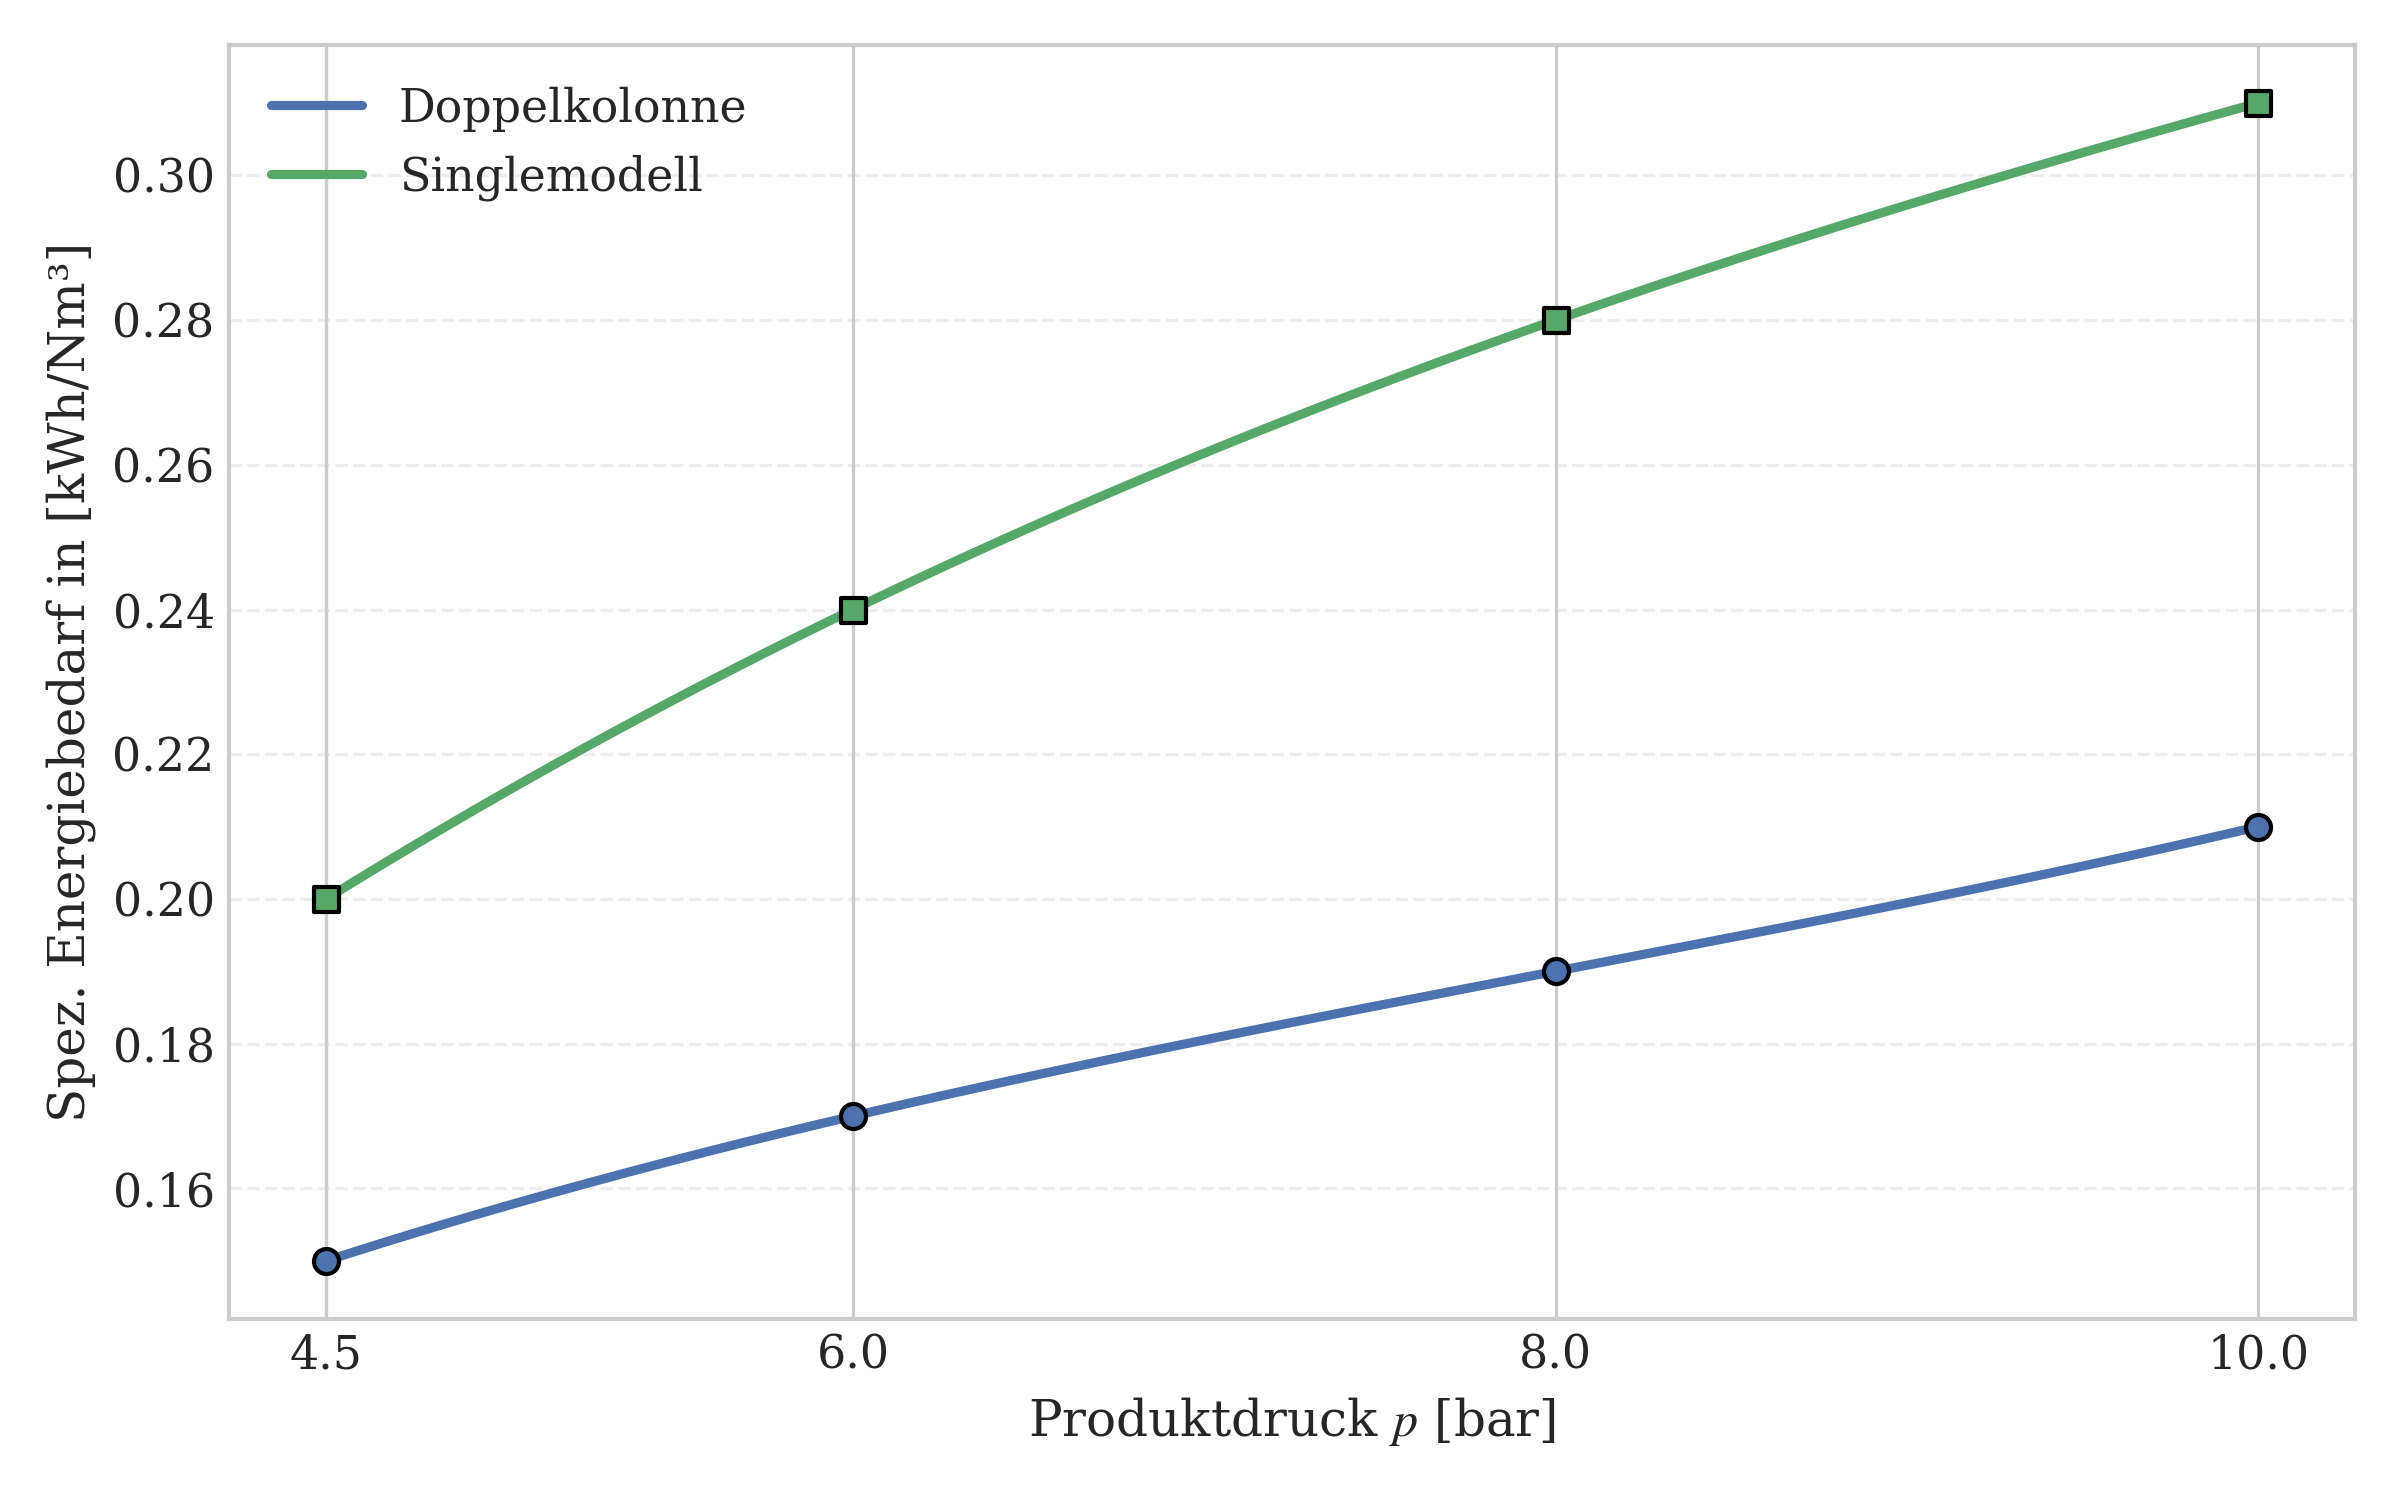
\includegraphics[width=0.8\textwidth]{Overleaf_LaTeX/bilder/vergleich_druckreihen_kwh_per_nm3.png}
    \caption{Spezifischer Energiebedarf des Single- und Doppelkolonnenmodells in Abhängigkeit des Produktdrucks}
    \label{fig:spez_energie_druck}
\end{figure}
\noindent
Der Vergleich der Simulationsdaten bei einem Referenzdruck von \SI{6}{bar} (abs.) verdeutlicht die signifikanten Unterschiede zwischen den beiden betrachteten Prozessvarianten. Für diesen Betriebspunkt wurde für das Einkolonnenmodell ein spezifischer Energiebedarf von \SI{0,2413}{kWh/Nm^3} ermittelt, während das Doppelkolonnenmodell einen Bedarf von \SI{0,1667}{kWh/Nm^3} aufweist. Dies entspricht einer energetischen Effizienzsteigerung des Doppelkolonnen-Konzepts von rund \SI{31}{\percent} gegenüber dem herkömmlichen Einkolonnen-Waste-Expander-Prozess. \\
Bezogen auf den Standardzustand (\SI{15}{\celsius}) belaufen sich die Werte auf \SI{0,2288}{kWh/m^3} für das Einkolonnenmodell und \SI{0,1580}{kWh/m^3} für das Doppelkolonnenmodell. Die detaillierten Stoffstromdaten und Zustandsgrößen für sämtliche Druckpunkte sind den Tabellen im Anhang \ref{tab:spez_energie_single, tab:spez_energie_doppel} im Normzustand ($0^\circ\text{C}$) und im Standardzustand ($15^\circ\text{C}$) zu entnehmen, um die Vergleichbarkeit mit Industriedaten zu gewährleisten. Unter Berücksichtigung der Normdichte von Stickstoff ergibt sich für das Singlemodell ein massenspezifischer Bedarf von \SI{0,1929}{kWh/kg_{N2}}, während das Doppelkolonnenmodell lediglich \SI{0,1333}{kWh/kg_{N2}} benötigt.
\begin{figure}[H]
    \centering
    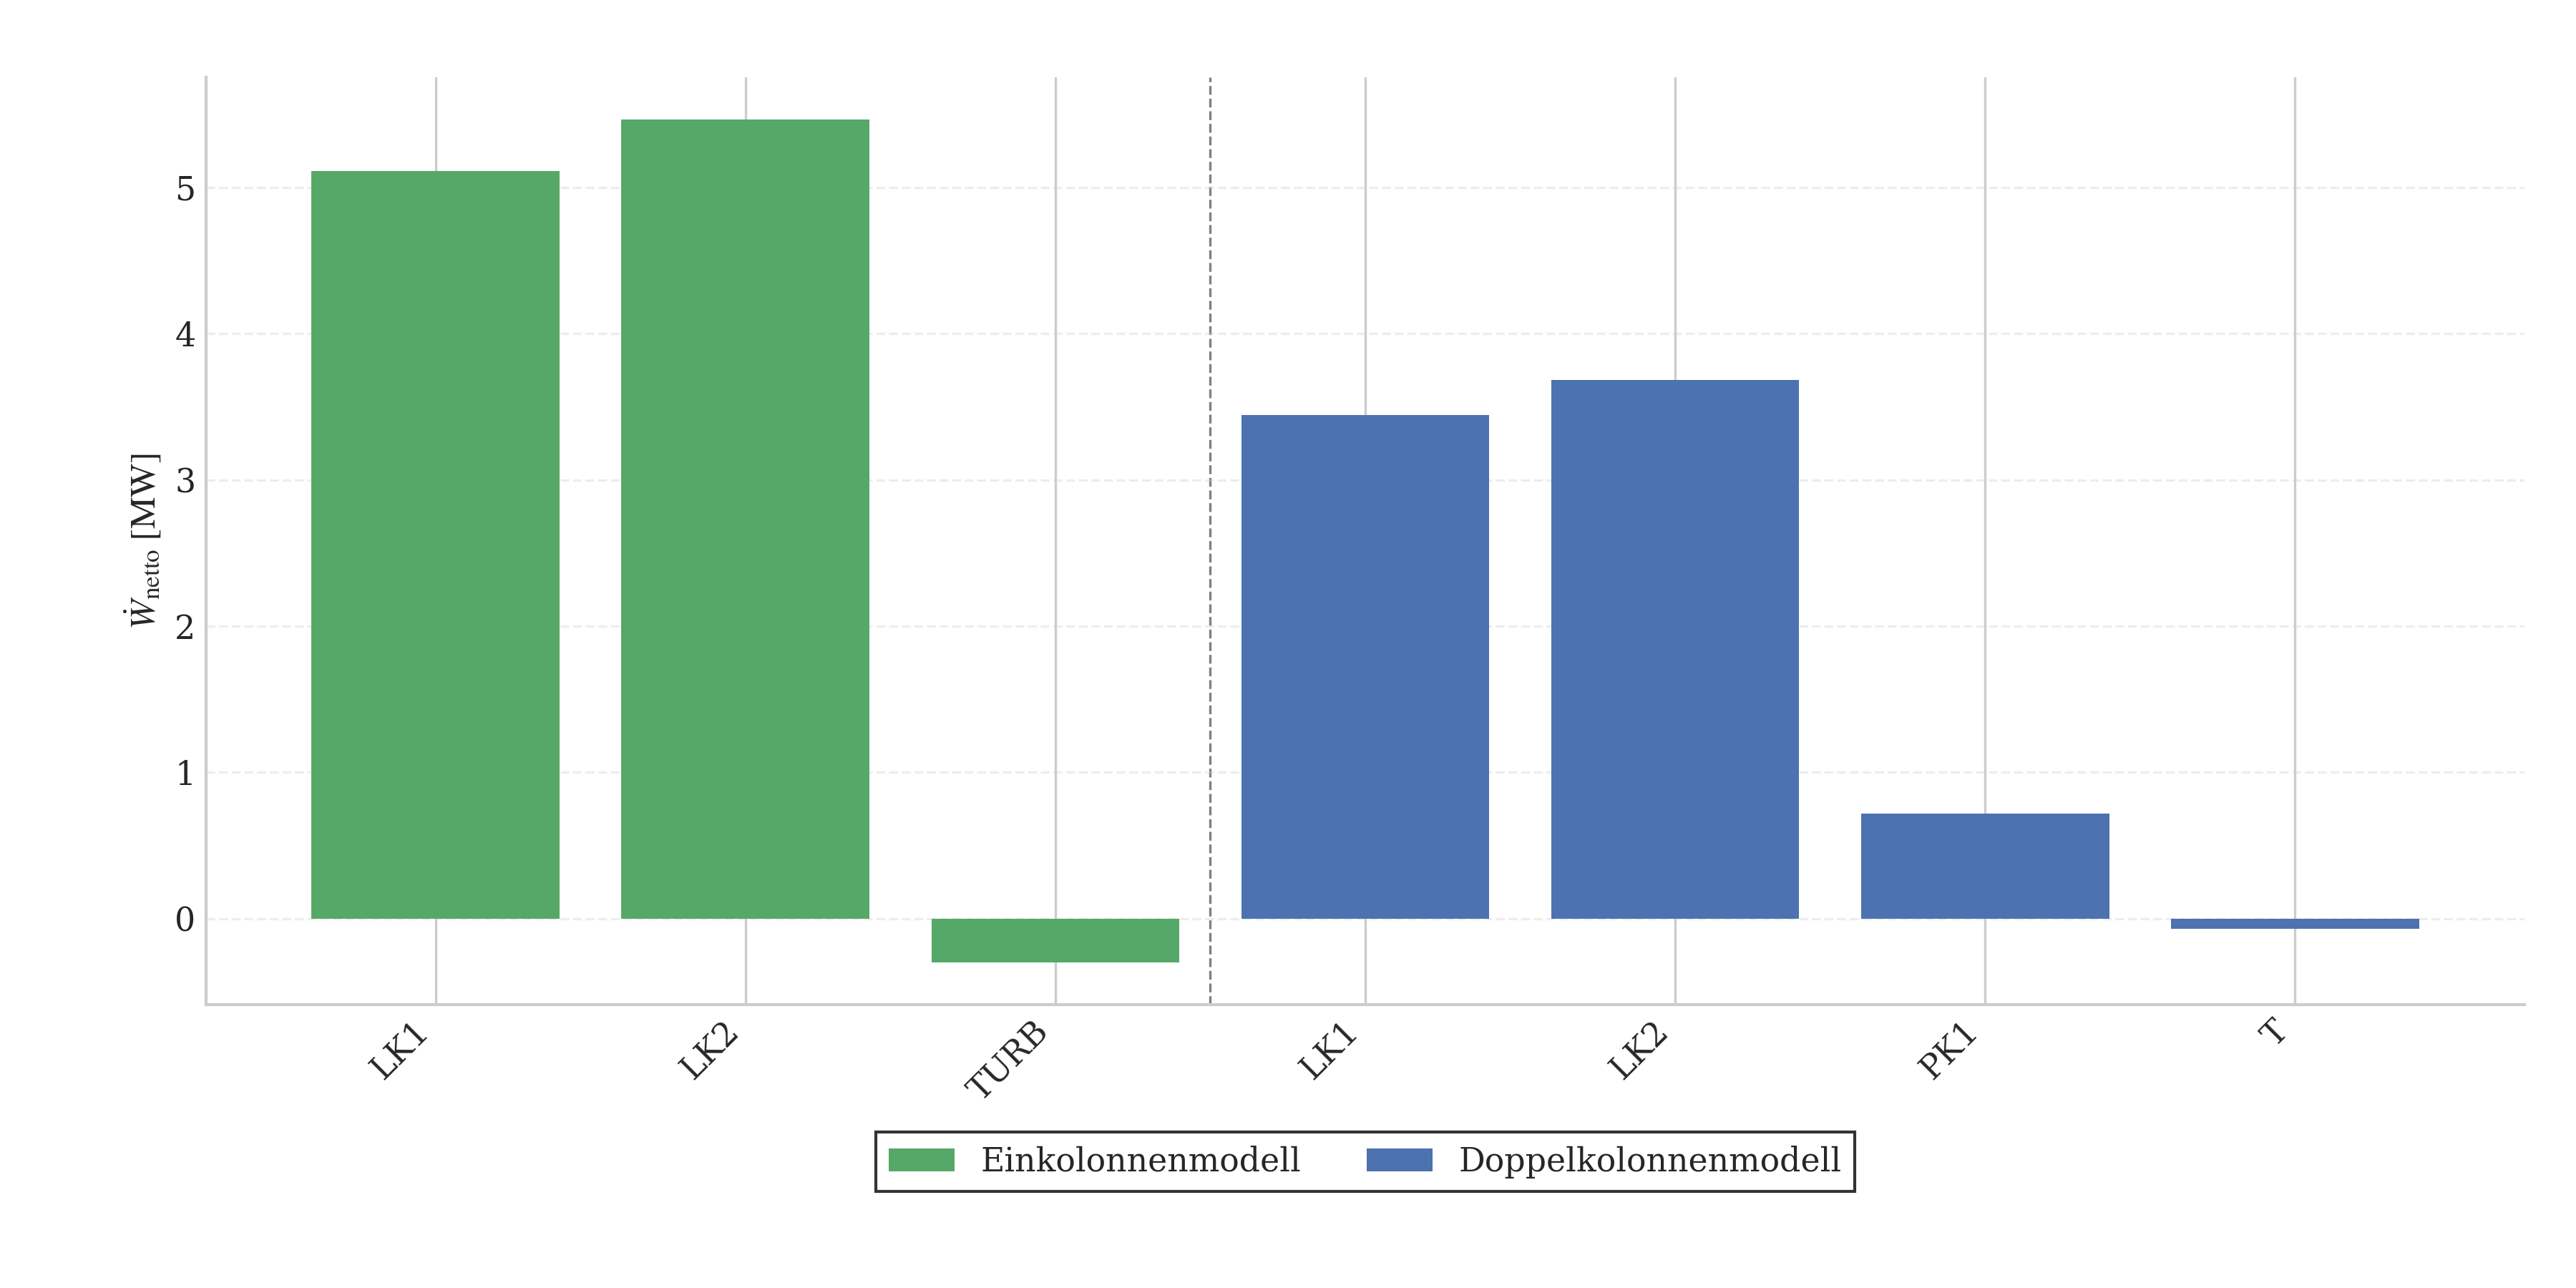
\includegraphics[width=0.8\textwidth]{Overleaf_LaTeX/bilder/vergleich_component_work_side_by_side.png}
    \caption{Vergleich der Leistungen der Verdichter- und Expansionseinheiten für das Single- und Doppelkolonnenmodell bei \SI{6}{bar}}
    \label{fig:vergleich_leistungen}
\end{figure}
\noindent
Abbildung \ref{fig:vergleich_leistungen} vergleicht die effektive Leistungsaufnahme (Net Work) der Verdichterstufen und Expansionsturbinen bei \SI{6}{bar}. Der deutlich höhere Luftbedarf des Einkolonnenmodells resultiert in einer massiv gesteigerten Leistungsaufnahme der Luftverdichter (LK1, LK2) von jeweils über \SI{5}{MW}. \\ Im Gegensatz dazu benötigt das Doppelkolonnenmodell für die Luftverdichtung lediglich ca. \SI{3,5}{MW} pro Stufe. Der zusätzliche Energieaufwand für den Produktverdichter (PK1) fällt mit unter \SI{1}{MW} gering aus und wird durch die Einsparungen bei der Hauptverdichtung überkompensiert. Während die Turbine im Einkolonnenmodell einen höheren Rückgewinnungsbeitrag leistet, ist die Turbinenleistung im Doppelkolonnen-Prozess aufgrund der optimierten Kälteintegration nahezu vernachlässigbar.\\ 
\\
Tabelle~\ref{tab:min_temp_approach_waermeuebertrager} zeigt die minimalen Temperaturabstände der betrachteten Wärmeübertrager für das Einkolonnen- und das Doppelkolonnenmodell. Berücksichtigt werden jeweils der Hauptwärmeübertrager sowie die im Modell enthaltenen Verdampfer-Kondensatoren. Die Werte wurden aus den Simulationsergebnissen der jeweiligen Apparate entnommen und dienen der Dokumentation der thermischen Annäherung innerhalb der Wärmeübertrager.\\
\begin{table}[H]
\centering
\caption{Minimaler Temperaturabstand der betrachteten Wärmeübertrager}
\label{tab:min_temp_approach_waermeuebertrager}
\begin{tabular}{llc}
\toprule
\textbf{Modellvariante} & \textbf{Wärmeübertrager} & \textbf{$\Delta T_\mathrm{min}$ [K]} \\
\midrule
Einkolonnenmodell      & MW  & 7{,}352 \\
Einkolonnenmodell      & RC  & 0{,}570 \\
Doppelkolonnenmodell   & MW  & 1{,}108 \\
Doppelkolonnenmodell   & RC1 & 0{,}504 \\
Doppelkolonnenmodell   & RC2 & 0{,}557 \\
\bottomrule
\end{tabular}
\end{table}

\section{Ergebnisse der Exergieanalyse}
\label{sec:ergebnisse_exergie}

Die exergetische Untersuchung der beiden Anlagenkonzepte zeigt deutliche Unterschiede in der Verteilung sowie der absoluten Höhe der Exergievernichtung. Während das Single-Kolonnenmodell eine Gesamtexergievernichtung von etwa \SI{6.9}{\mega\watt} aufweist, liegt dieser Wert beim Doppelkolonnenmodell mit circa \SI{4.2}{\mega\watt} deutlich niedriger.\\
Im Single-Kolonnenmodell konzentriert sich die Exergievernichtung auf wenige Hauptkomponenten, wobei der Hauptwärmeübertrager MH mit \SI{1.806}{\mega\watt} die größte Einzelquelle für Exergieverluste darstellt. Dies entspricht einem Anteil von nahezu 20\,\% an der gesamten Vernichtung innerhalb dieses Modells (vgl. Anhang \ref{fig:exergieverluste_einzelkolonne, fig:exergieverluste_doppelkolonne}. Durch Anpassung des minimalen Temperaturabstands im Multistromwärmeübertrager ist es Möglich die Exergievernichtung des Wärmeübertragers zu verringern auf Kosten der Vernichtung in der Drossel D2. Dieser Zusammenhang ist im Anhang in der Auswertung in Abbildung \ref{fig:exergieverluste_einzelkolonne_zusatz} zu erkennen.\\
Auch die Zwischenkühler ZK1 und ZK2 tragen zusammen mit rund \SI{2.07}{\mega\watt} massiv zur Entropieproduktion bei. Da deren exergetischer Wirkungsgrad definitionsgemäß bei Null liegt, geht hier das gesamte Exergiepotential der Abwärme an die Umgebung verloren.\\
Trotz eines relativ hohen Bauteilwirkungsgrads von etwa 89\,\% gehören die Luftverdichter LK1 und LK2 zu den wesentlichen Vernichtungsträgern. \\
Das Doppelkolonnenmodell zeigt eine gleichmäßigere Verteilung der Verluste auf eine größere Anzahl an Komponenten, wobei die absoluten Spitzenwerte deutlich unter denen des Single-Modells liegen. Auch in diesem Fall sind die Zwischenkühler ZK2 mit \SI{0.780}{\mega\watt} und ZK1 mit \SI{0.577}{\mega\watt} sowie der Hauptwärmeübertrager MW mit \SI{0.502}{\mega\watt} die dominierenden Komponenten. Im Vergleich zum Single-Modell konnte die Vernichtung im Hauptwärmeübertrager jedoch stark reduziert werden.\\
Das Modell teilt die Trennung auf zwei Kolonnen auf, wobei die Niederdruckkolonne KOLLP mit \SI{0.466}{\mega\watt} eine deutlich höhere Exergievernichtung als die Hochdruckkolonne KOLHP mit \SI{0.152}{\mega\watt} verursacht. Die Hochdruckkolonne arbeitet dabei mit einem sehr hohen exergetischen Wirkungsgrad von 97\,\%.\\
Die Exergievernichtung in den Hauptverdichtern LK1 und LK2 reduziert sich im Doppelkolonnenmodell auf jeweils etwa \SI{0.396}{\mega\watt}. In beiden Modellen bilden die thermischen Apparate die größte Gruppe der Exergievernichter.\\

\begin{figure}[H]
    \centering
    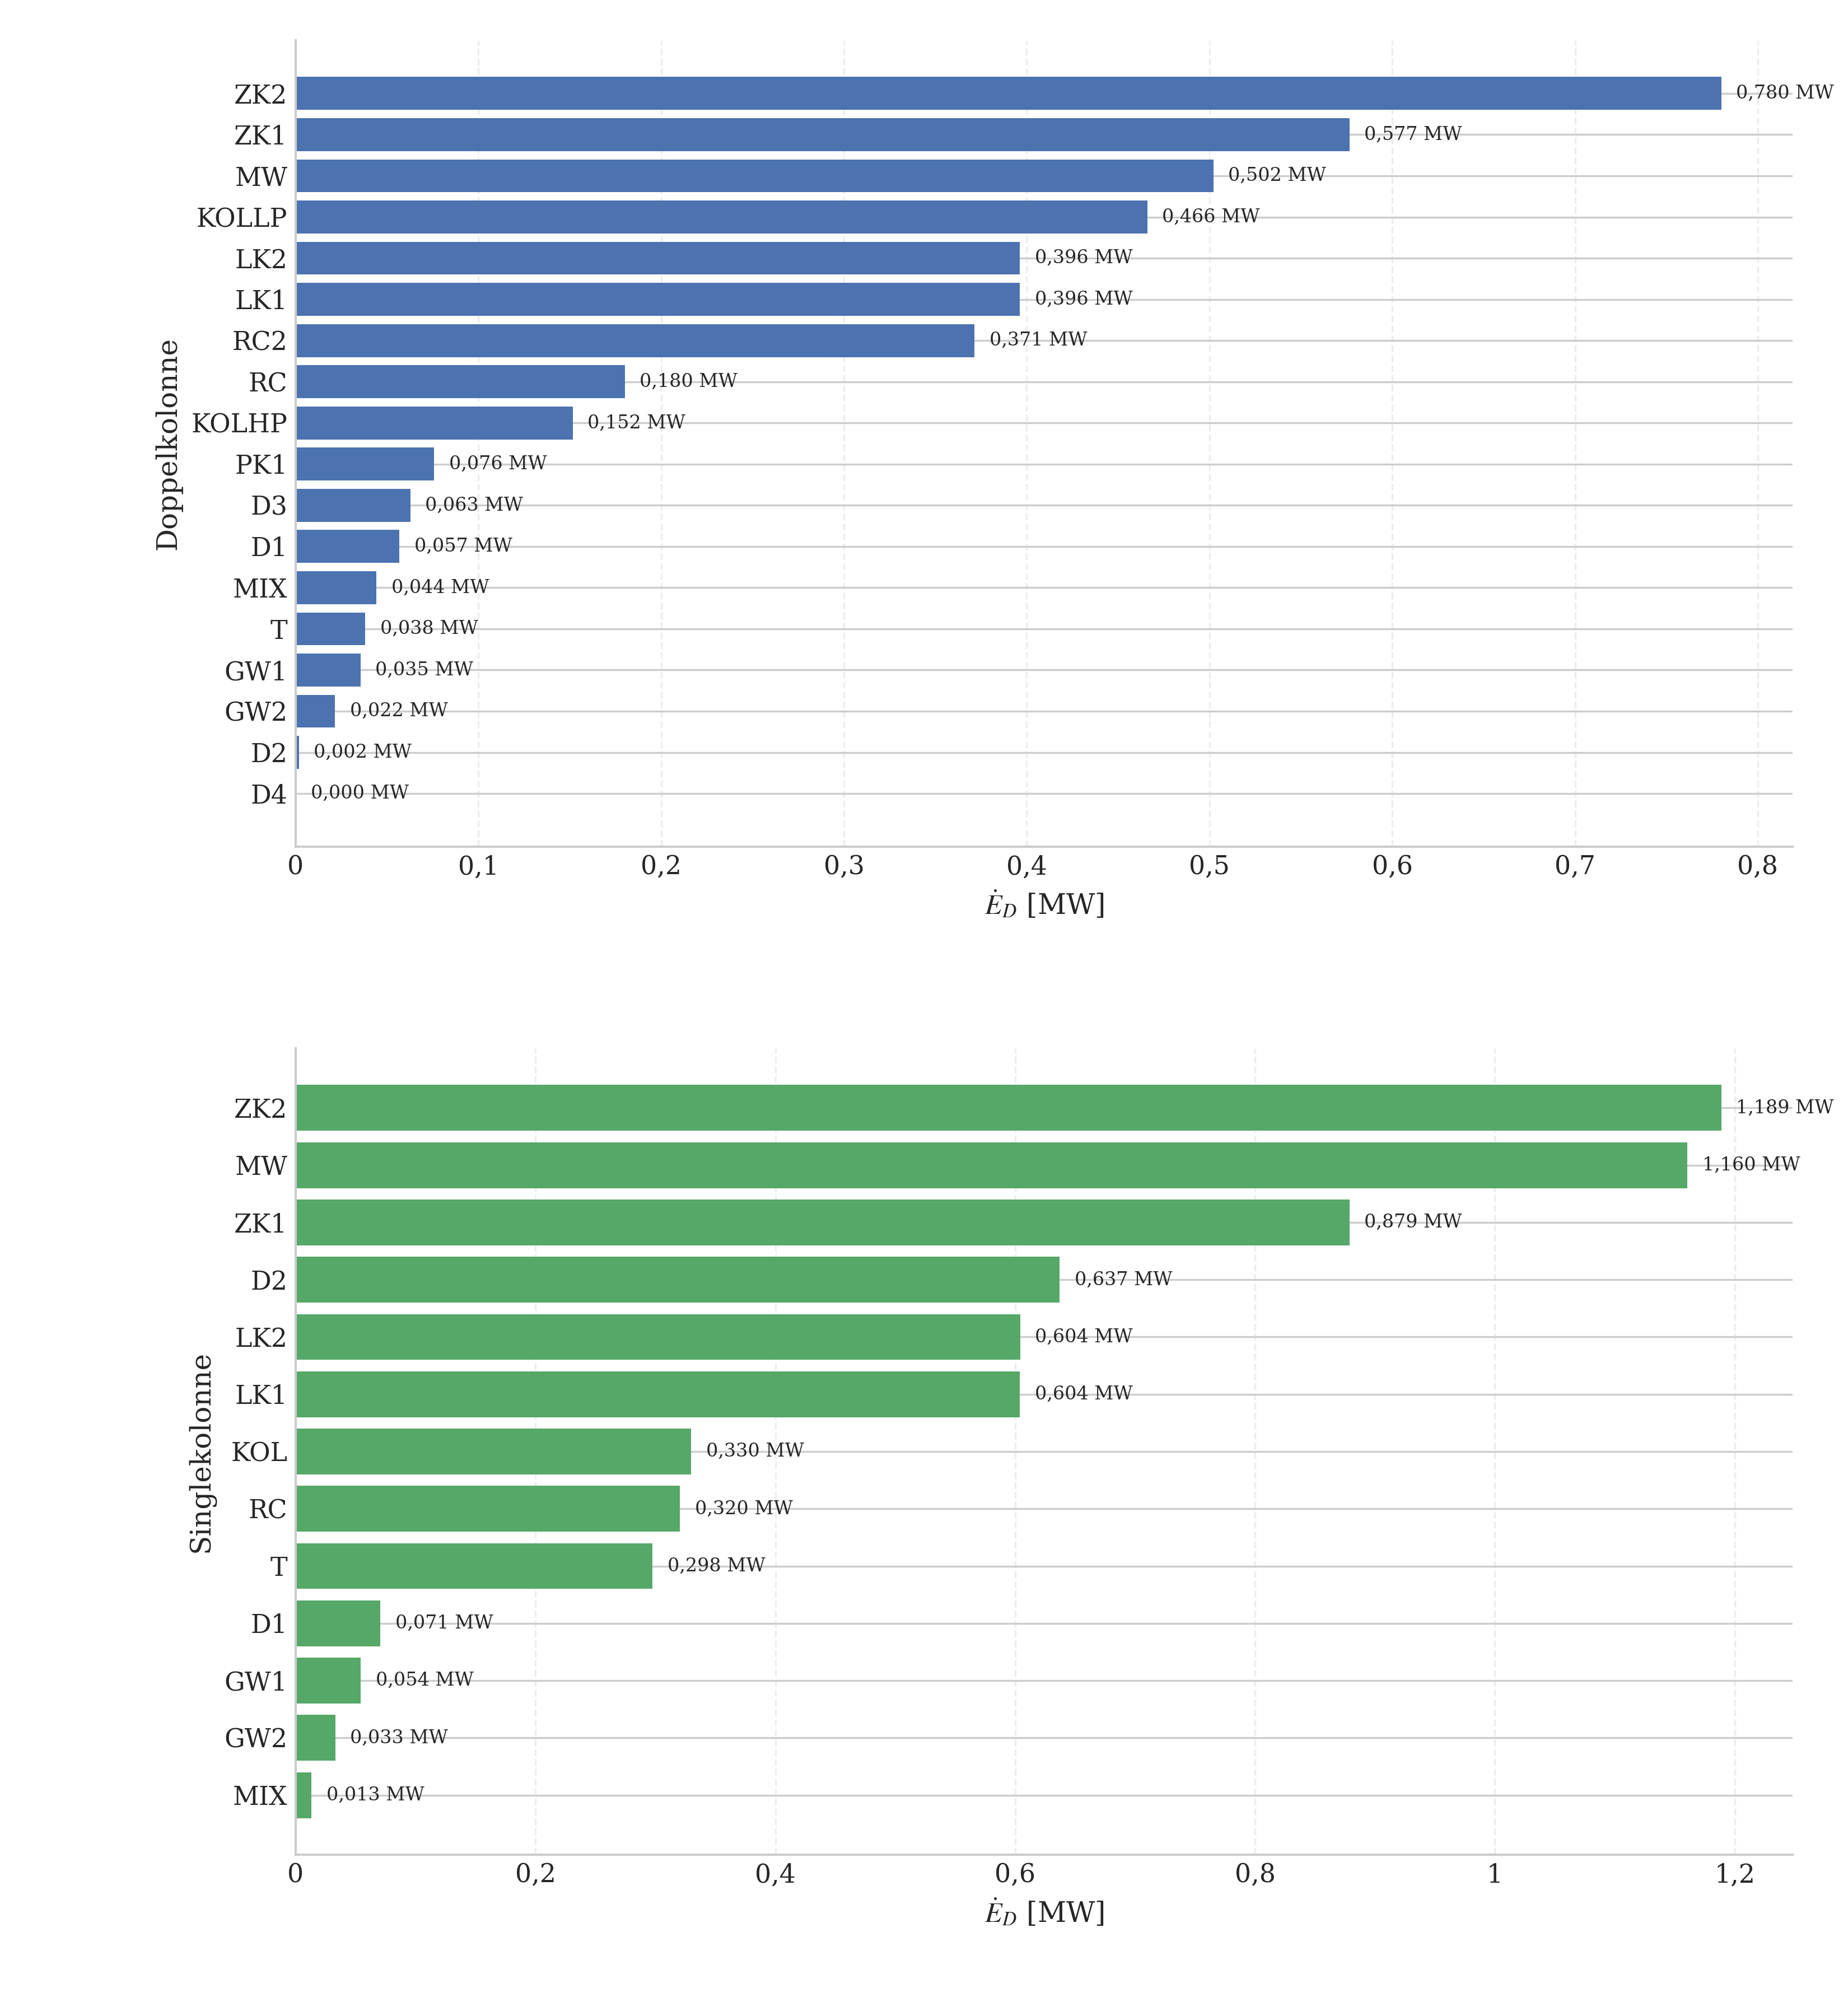
\includegraphics[width=0.9\textwidth]{Overleaf_LaTeX/bilder/vergleich_component_pareto_ED.png}
    \caption{Vergleich der Exergievernichtung $\dot{E}_D$ der Systemkomponenten im Doppelkolonnenprozess (oben) und Einzelkolonnenprozess (unten). Die Darstellung verdeutlicht die unterschiedlichen Hauptquellen irreversibler Verluste in beiden Prozesskonfigurationen.}
    \label{fig:exergiedestruktion_vergleich}
\end{figure}

\noindent
Die Analyse der relativen Exergiedestruktion $y_{D,b}$ auf Ebene der Hauptprozessblöcke verdeutlicht die unterschiedliche Gewichtung der Verlustquellen zwischen dem Einzelkolonnen- und dem Doppelkolonnenmodell. Für beide Konfigurationen identifiziert der Verdichtungs- und Gasaufbereitungsblock (V+G-Block) den Bereich mit dem größten Anteil an der gesamten Exergievernichtung. Beim Doppelkolonnenmodell liegt dieser Wert mit etwa 55\,\% signifikant höher als beim Einzelkolonnenmodell, welches dort knapp 50\,\% erreicht.\\
Innerhalb dieses Blocks zeigt sich für beide Modelle eine ähnliche interne Aufteilung, die Kompression jeweils einen deutlich größeren Beitrag leistet die Reinigung. Im Doppelkolonnenmodell entfallen circa 35\,\% auf die Kompression und etwa 20\,\% auf die Reinigung, während im Einzelkolonnenmodell die Kompression bei rund 31\,\% und die Reinigung bei etwa 19\,\% liegen.\\
Im Bereich der Wärmeübertrager zeigen sich die gravierendsten Unterschiede in der relativen Relevanz der Verluste. Während der Wärmeübertragerblock im Einkolonnenmodell mit etwa 27\,\% die zweitgrößte Verlustquelle darstellt, reduziert sich dieser Anteil im Doppelkolonnenmodell auf lediglich etwa 12\,\%.\\
Ein umgekehrtes Bild ergibt sich beim Kolonnenblock. Hier verursacht das Doppelkolonnenmodell mit rund 30\,\% einen wesentlich höheren Anteil an der relativen Exergiedestruktion als das Einzelkolonnenmodell, dessen Kolonnenblock lediglich für etwa 12\,\% der Verluste verantwortlich ist.\\
Die unter der Kategorie Rest zusammengefassten übrigen Komponenten spielen im Doppelkolonnenmodell fast keine Rolle für die gesamte Exergievernichtung. Im Gegensatz dazu weist das Einzelkolonnenmodell in dieser Kategorie einen nennenswerten Beitrag von etwa 14\,\% auf, was die exergetische Relevanz der Zusatzkomponenten des Waste-Expanders unterstreicht.\\

\begin{figure}[H]
    \centering
    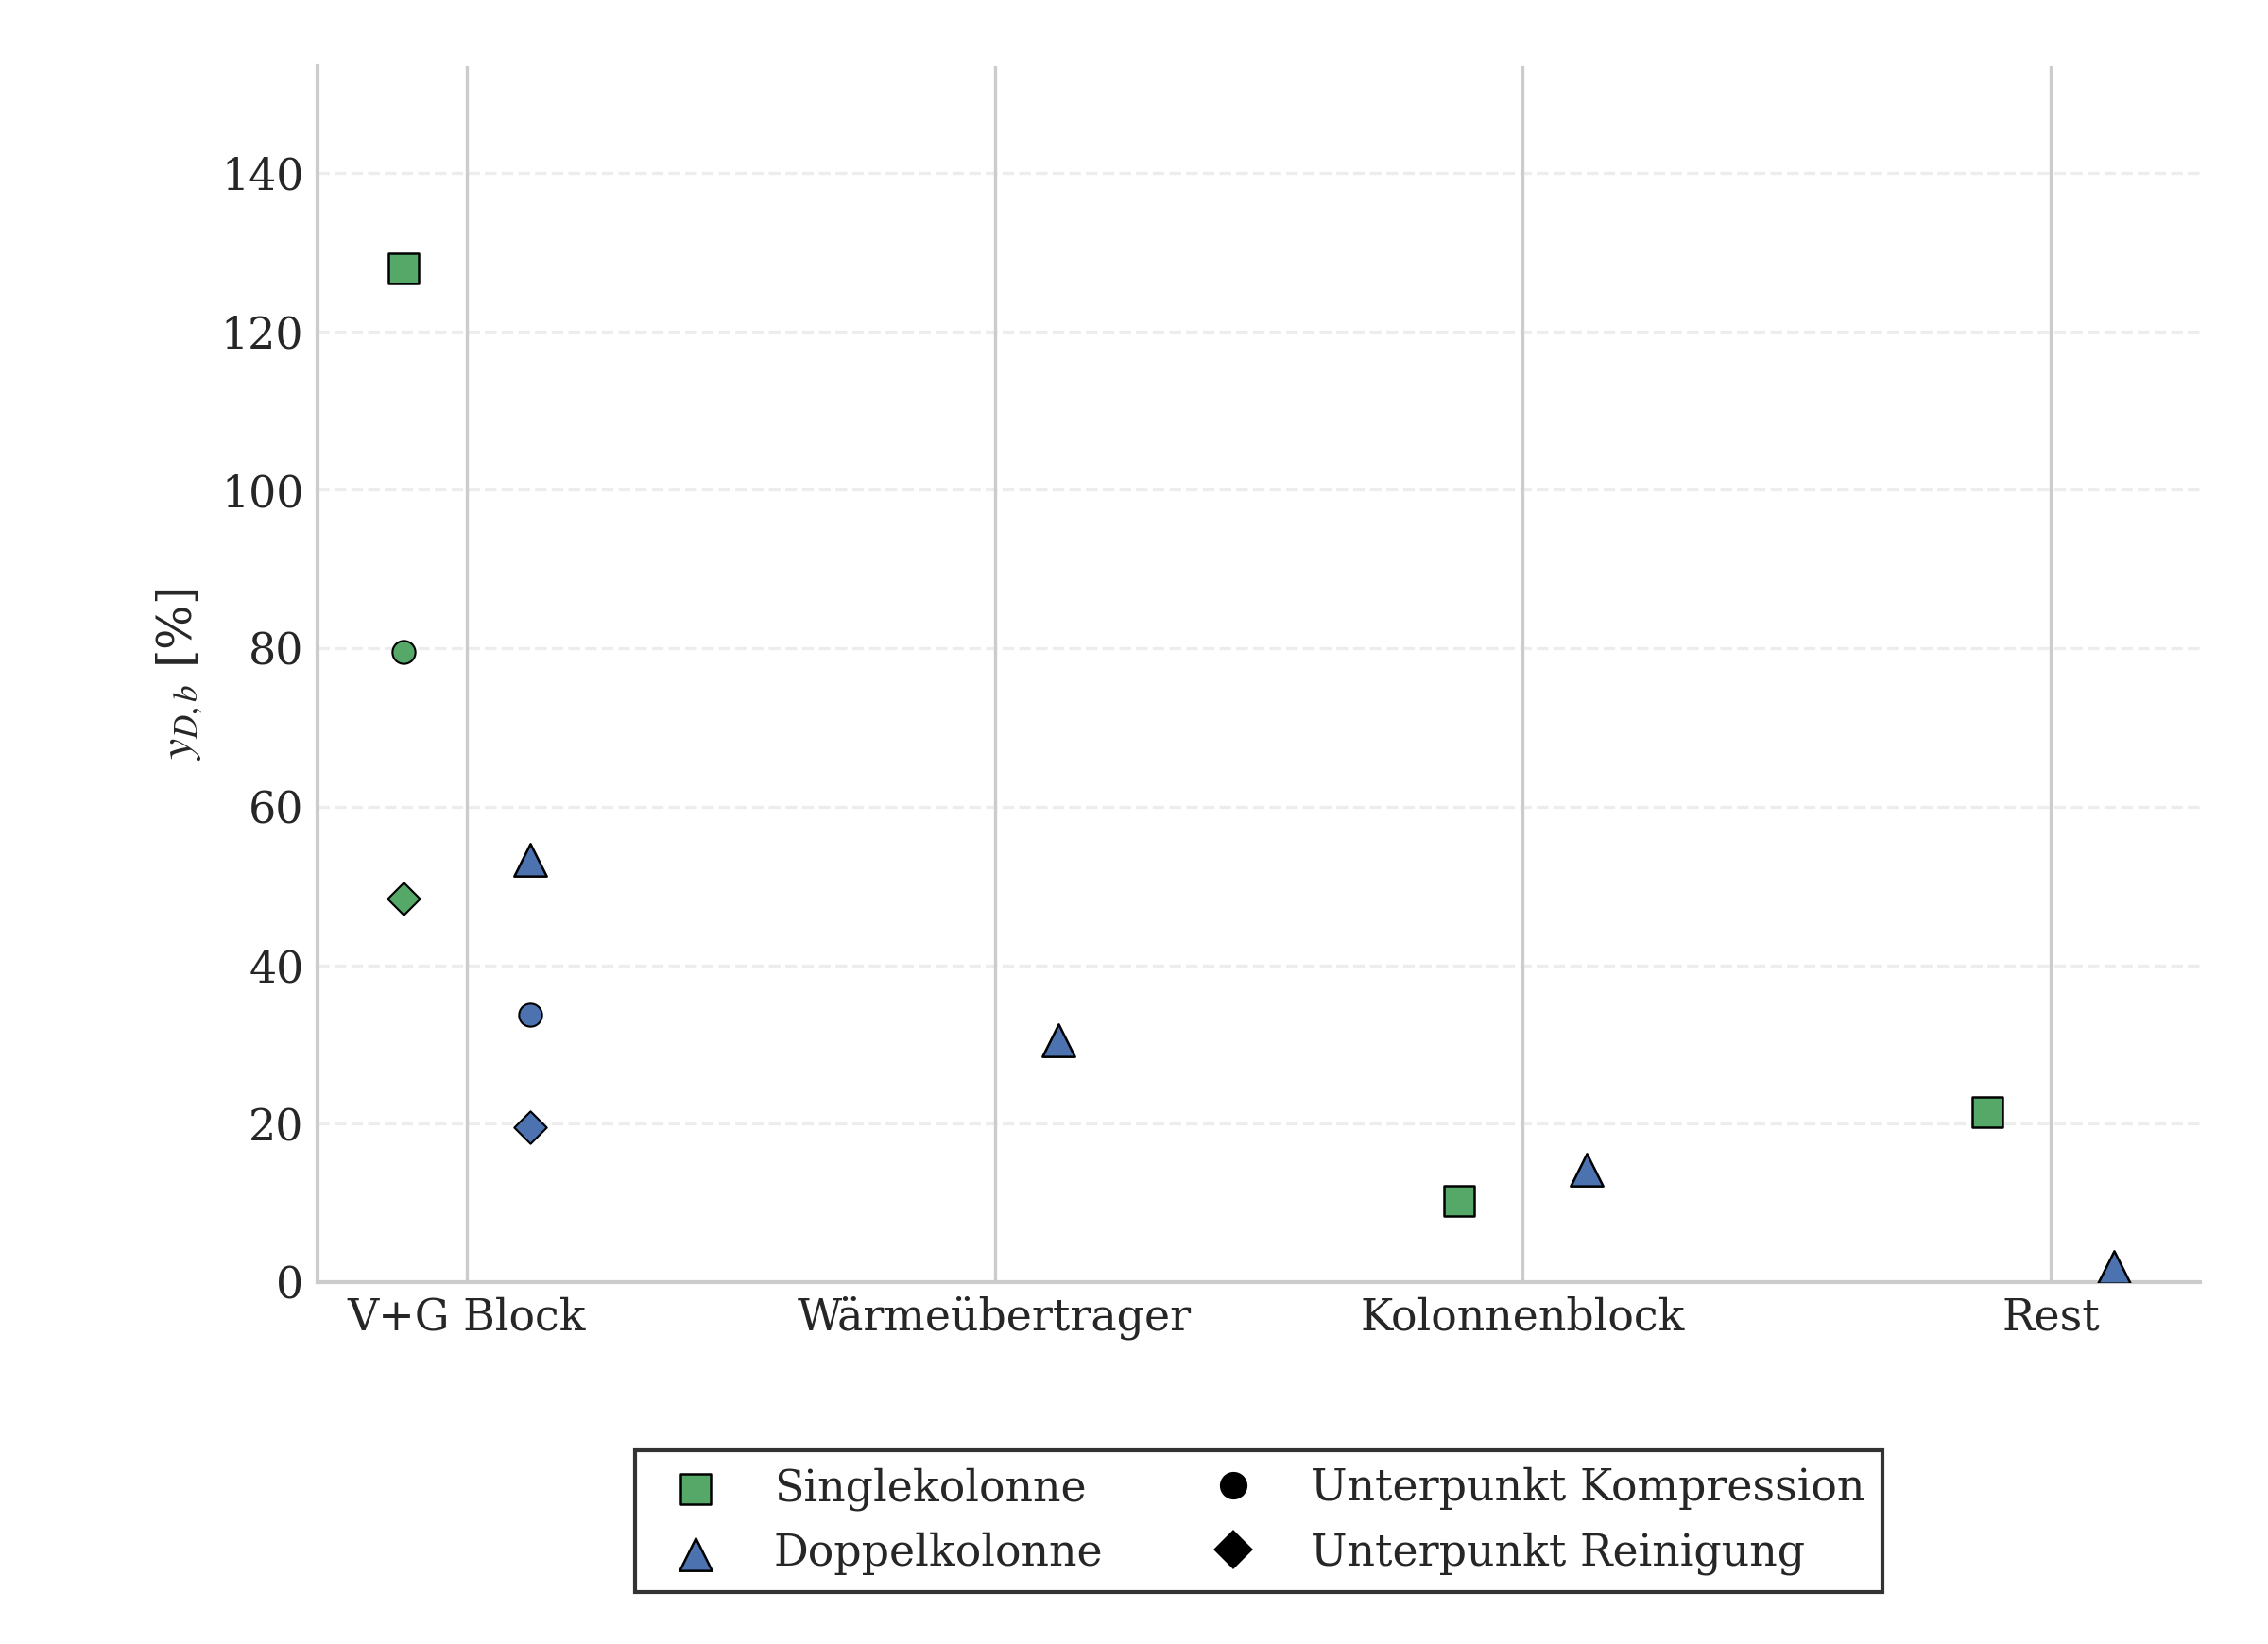
\includegraphics[width=0.8\textwidth]{Overleaf_LaTeX/bilder/vergleich_yD_funktionsbloecke.png}
    \caption{Vergleich der relativen Exergiedestruktion $y_{D,b}$ der Hauptprozessblöcke für das Einzelkolonnen- und Doppelkolonnenmodell. Dargestellt sind die Beiträge des Verdichtungs- und Gasaufbereitungsblocks (V+G Block), der Wärmeübertrager, des Kolonnenblocks sowie der übrigen Komponenten (Rest). Die Markierungen kennzeichnen zusätzlich die Unterpunkte Kompression und Reinigung innerhalb des V+G Blocks.}
    \label{fig:vergleich_exergiedestruktion_bloecke}
\end{figure}
\noindent
Der abschließende Vergleich der Exergiebilanzen beider Prozesskonfigurationen verdeutlicht die Überlegenheit des Doppelkolonnenmodells hinsichtlich des Aufwands und der prozessinternen Effizienz. Der gesamte Exergieaufwand $\dot{E}_{F,tot}$ fällt für das Doppelkolonnenmodell mit \SI{7.768}{\mega\watt} wesentlich geringer aus als für das Single-Kolonnenmodell, welches einen Input von \SI{10.757}{\mega\watt} benötigt.\\
Bei der resultierenden Produktexergie $\dot{E}_{P,tot}$ liegen beide Modelle hingegen nah beieinander, wobei das Single-Kolonnenmodell mit \SI{3.310}{\mega\watt} einen leicht höheren Wert erreicht als das Doppelkolonnenmodell mit \SI{2.975}{\mega\watt}. Trotz dieses geringeren absoluten Nutzens weist das Doppelkolonnenmodell mit 38{,}30\,\% einen deutlich höheren exergetischen Wirkungsgrad $\eta_{ex}$ auf als das Single-Kolonnenmodell, welches eine Effizienz von 30{,}77\,\% erreicht.\\
Die Ursache hierfür liegt neben dem Aufwand in der massiven Reduktion der totalen Exergievernichtung $\dot{E}_{D,tot}$ von circa \SI{6.95}{\mega\watt} im Single-Kolonnenmodell auf \SI{4.23}{\mega\watt} im Doppelkolonnenmodell.\\
Die externen Exergieverluste $\dot{E}_{L,tot}$ zeigen in beiden Modellen mit \SI{0.505}{\mega\watt} beziehungsweise \SI{0.487}{\mega\watt} ähnliche Werte. \\

\begin{figure}[H]
    \centering
    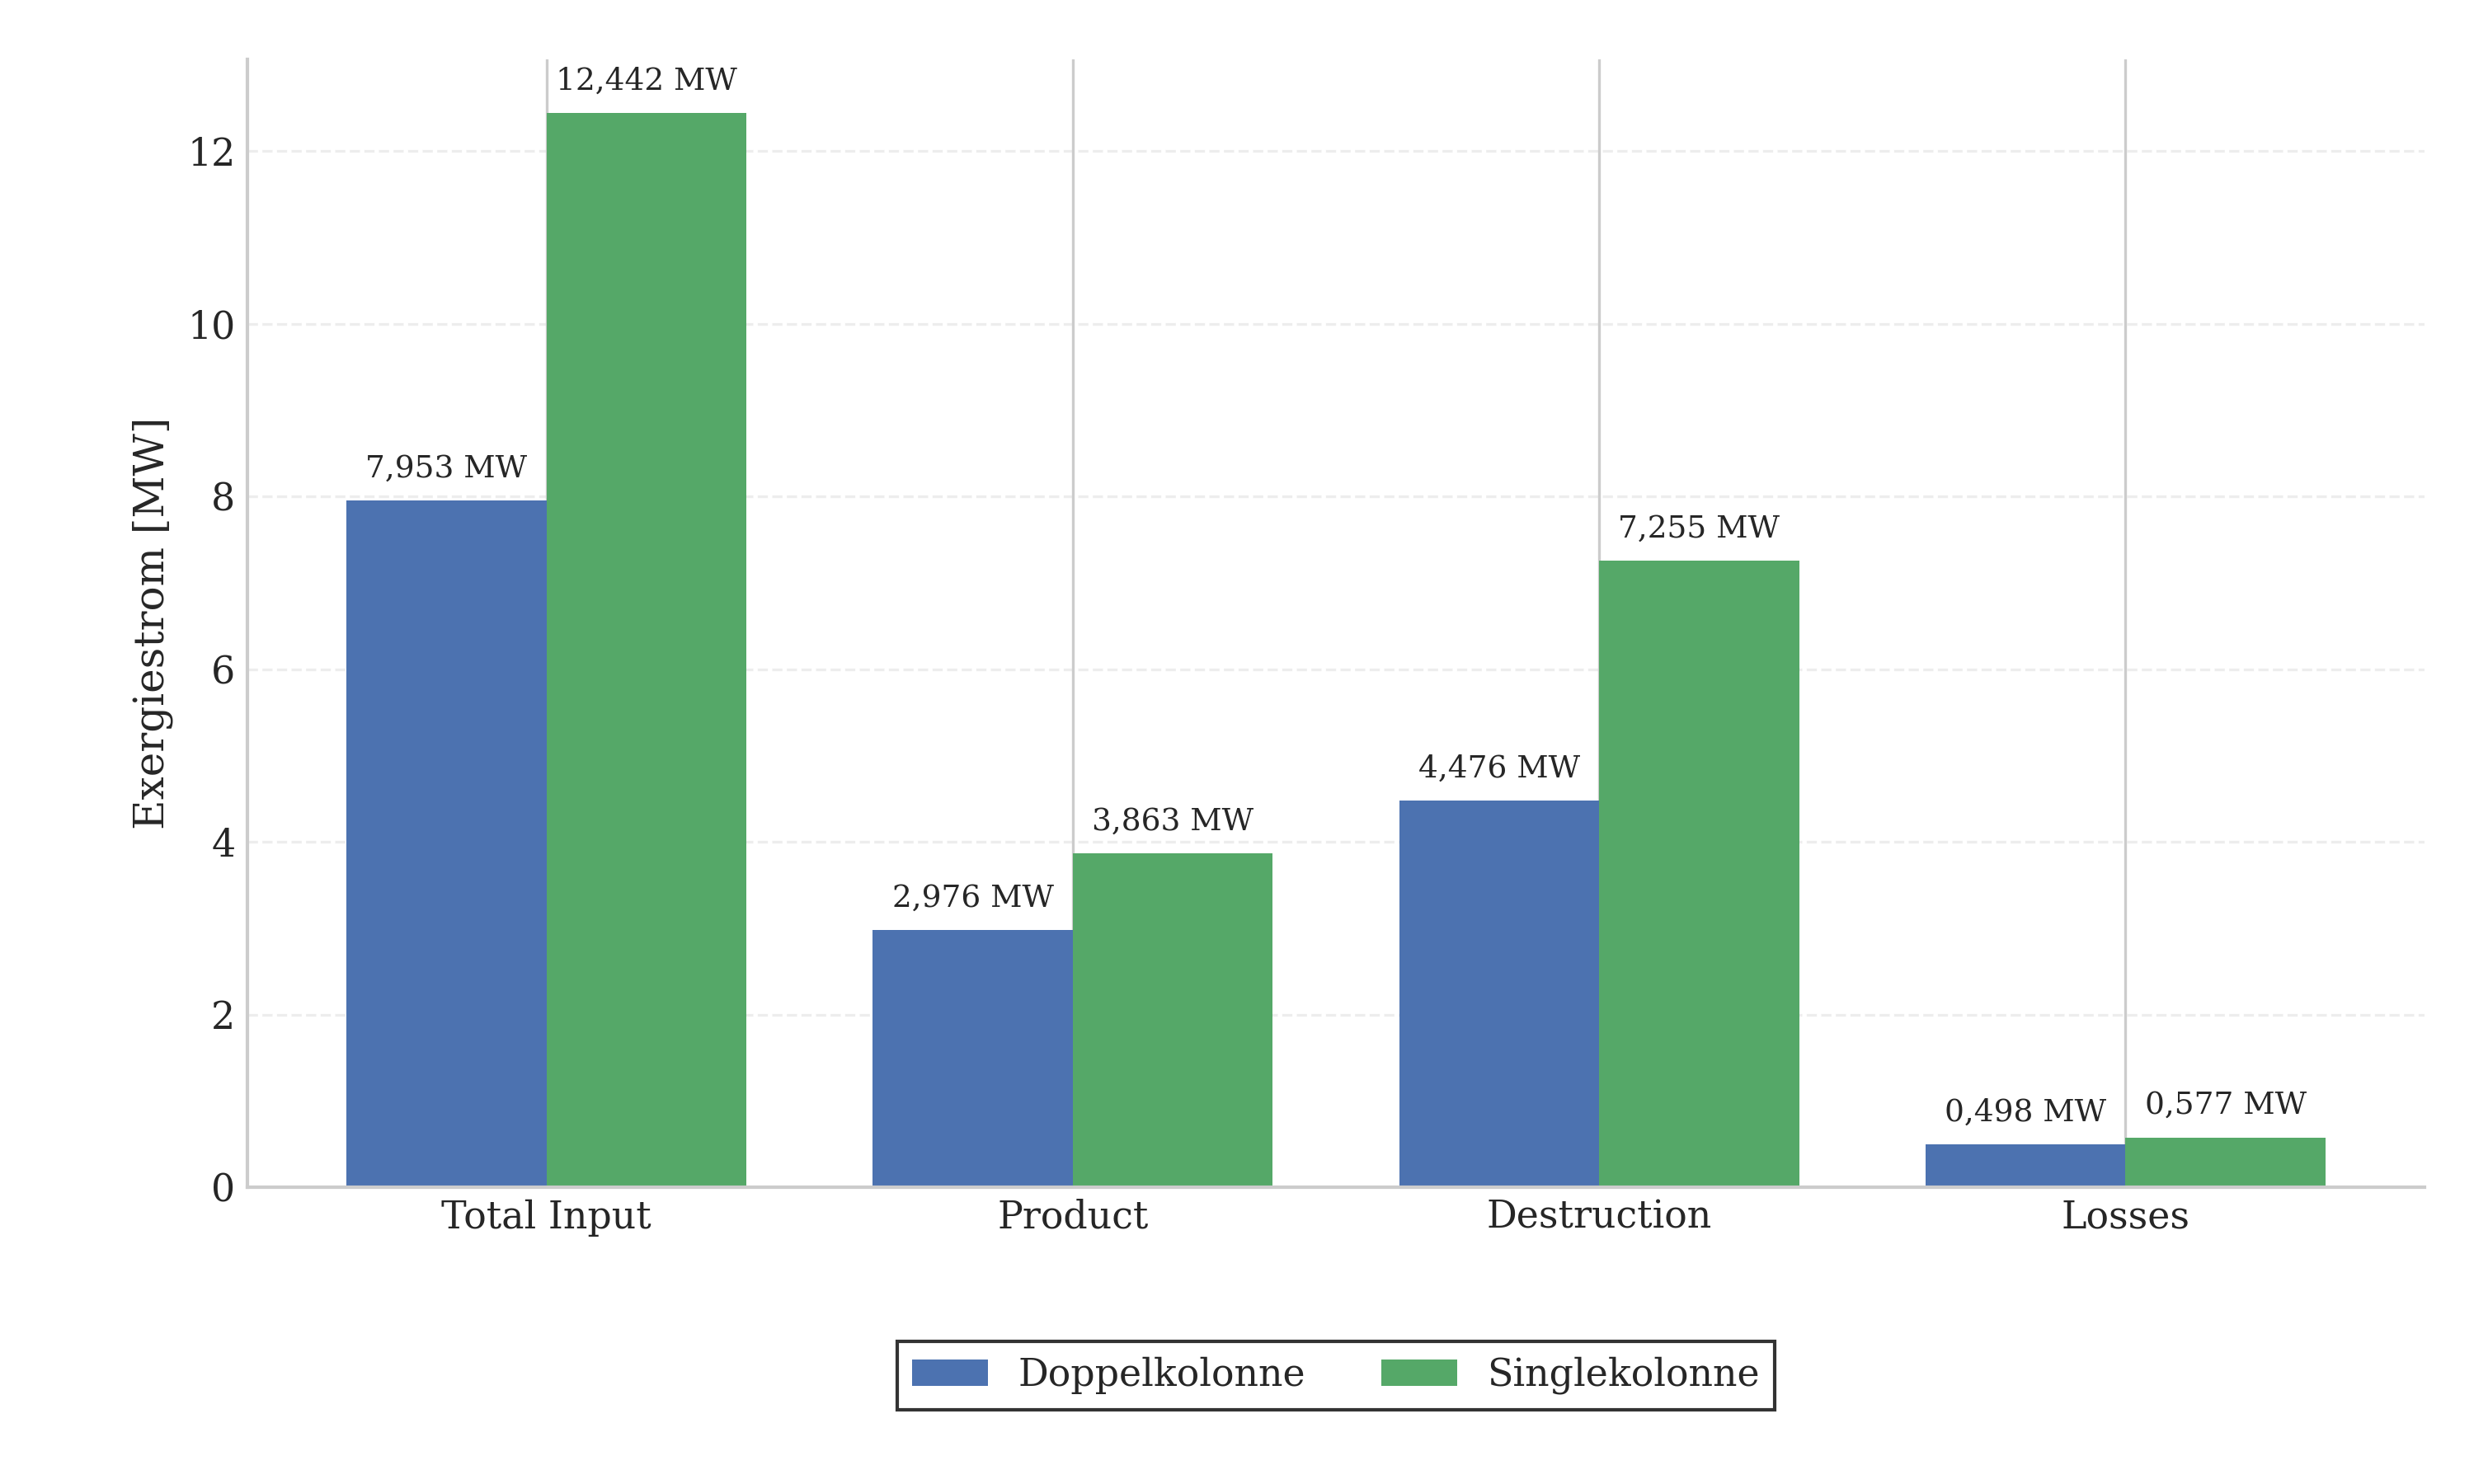
\includegraphics[width=0.9\textwidth]{Overleaf_LaTeX/bilder/vergleich_global_kennzahlen_grouped.png}
    \caption{Vergleich der Exergiebilanz beider Prozesskonfigurationen. Dargestellt sind Gesamt-Exergieinput $\dot{E}_F$, Produkt-Exergie $\dot{E}_P$, Exergiedestruktion $\dot{E}_D$ sowie Exergieverluste $\dot{E}_L$ für den Doppelkolonnen- und Einzelkolonnenprozess.}
    \label{fig:exergiebilanz_vergleich}
\end{figure}

\section{Ergebnisse der wirtschaftlichen Auswertung}
\label{sec:ergebnisse_wirtschaft}


Die wirtschaftliche Bewertung der untersuchten Prozessvarianten erfolgt auf
Basis der Investitionskosten, des jährlichen Total Revenue Requirement
\(TRR_L\) sowie der spezifischen Stickstoffbereitstellungskosten \(c_{N_2}\).
Die Ergebnisse werden für das Einkolonnenmodell und das Doppelkolonnenmodell
jeweils in einer kleinen und einer großen Auslegungsvariante gegenübergestellt.
Dabei repräsentiert die kleine Variante den geforderten Produktmassenstrom von
\(\dot{m}_{N_2}=\SI{4.65}{\kilogram\per\second}\), während die große Variante
einen Produktmassenstrom von \(\dot{m}_{N_2}=\SI{15.01} {\kilogram\per\second}\) abbildet. Auf dieser Grundlage werden zunächst die Investitionskosten und anschließend die jährlichen sowie spezifischen Bereitstellungskosten ausgewertet. Die Kosten werden in EUR$_{2026}$ angegeben.\\
\\
Die zusammengefassten Investitionskosten der untersuchten Prozessvarianten sind
in Tabelle~\ref{tab:investitionskosten_zusammenfassung} dargestellt. Die
detaillierte Herleitung der einzelnen Kostenpositionen erfolgt im
Anhang~\ref{ch:a_kosten}. Dort werden die apparatespezifischen Kosten für
Verdichter, Expander, Wärmeübertrager und Kolonnen zunächst einzeln bestimmt
und anschließend in Bare-Module-Kosten überführt. Auf dieser Grundlage werden
die Kosten der Hauptapparate, der Kolonnenblock sowie die pauschal angesetzte
Luftvorreinigung zu den gesamten Investitionskosten zusammengeführt. \\
In Tabelle~\ref{tab:investitionskosten_zusammenfassung} ist zu erkennen, dass die Investitionskosten mit zunehmender Anlagengröße deutlich ansteigen. Für beide Anlagengrößen liegen die Kosten des Doppelkolonnenmodells über denen des Einkolonnenmodells. Der größte Kostenbeitrag ergibt sich in allen Varianten aus den Bare-Module-Kosten der Hauptapparate. Zu beachten ist in dieser Tabelle, dass die Kosten, welche die Kolonne zu den gesamten Investitionskosten beiträgt, der reine Kolonnenkörper ohne Verdampfer und Kondensator darstellt. Die gekoppelten Verdampfer-Kondensator-Apparate werden in den Hauptapperaten als individuelle Komponenten berechnet. Die Luftvorreinigung wird pauschal als Zuschlag auf die Hauptapparatekosten berücksichtigt.
Das Total Capital Investment ergibt sich anschließend aus dem Fixed Capital Investment unter Berücksichtigung der in der wirtschaftlichen Modellierung definierten Zuschläge (vgl. Kapitel \ref{sec:modell_economics}.

\begin{table}[H]
\centering
\caption{Zusammenfassung der Investitionskosten der untersuchten Varianten}
\label{tab:investitionskosten_zusammenfassung}
\small
\setlength{\tabcolsep}{5pt}
\begin{tabular}{l
                S[table-format=8.0]
                S[table-format=8.0]
                S[table-format=8.0]
                S[table-format=8.0]}
\toprule
\textbf{Kostenposition}
& \multicolumn{2}{c}{\textbf{Einkolonnenmodell}}
& \multicolumn{2}{c}{\textbf{Doppelkolonnenmodell}} \\
\cmidrule(lr){2-3}
\cmidrule(lr){4-5}
& {\textbf{klein}}
& {\textbf{groß}}
& {\textbf{klein}}
& {\textbf{groß}} \\
\midrule
&\multicolumn{4}{c}{\textit{Kosten in EUR$_{2026}$}} \\
\midrule
PEC-Summe Hauptapparate
& 1408580 & 3113923 & 1688732 & 4125069 \\
Bare-Module-Kosten Hauptapparate
& 3605965 & 7971642 & 4323152 & 10560177 \\
Kolonnenblock
& 1091900 & 2492300 & 1884700 & 4006700 \\
Luftvorreinigung
& 375829 & 837115 & 496628 & 1165350 \\
\midrule
FCI
& 6864708 & 15290331 & 9071161 & 21285703 \\
TCI
& 10091121 & 22476787 & 13334607 & 31289983 \\
\bottomrule
\end{tabular}
\end{table}

\begin{figure}[H]
\centering
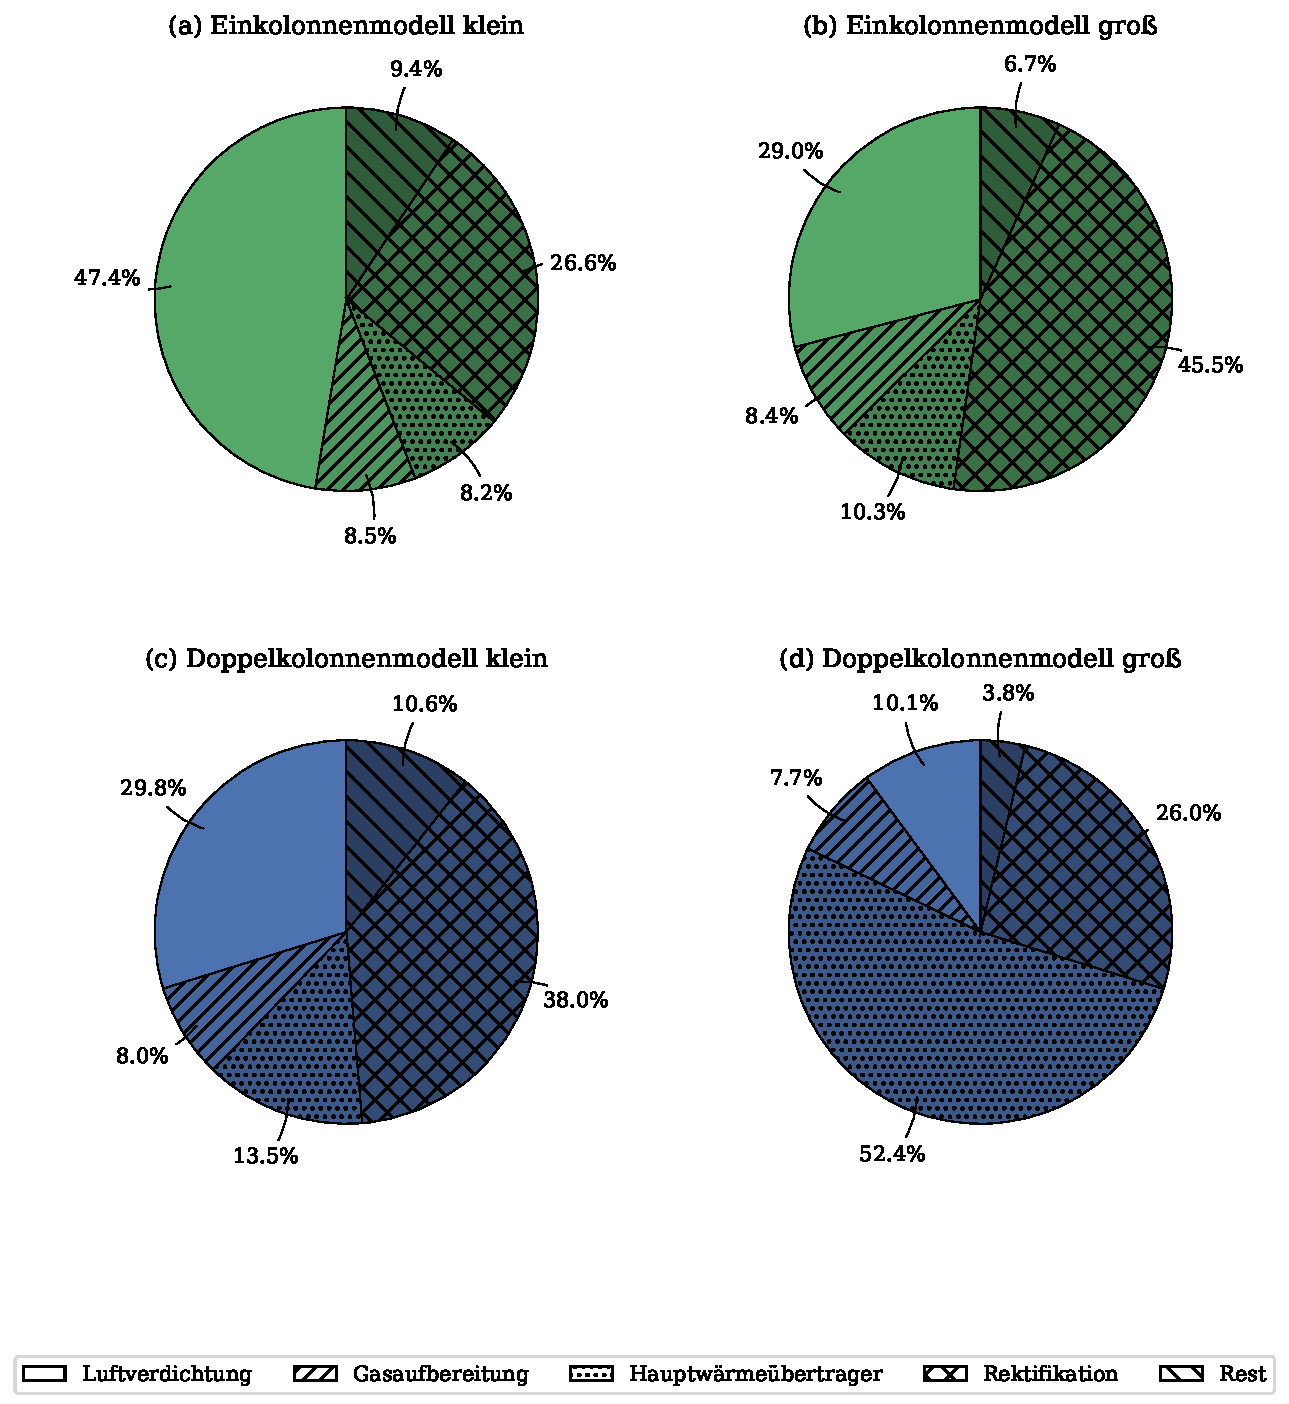
\includegraphics[width=0.95\textwidth]{Overleaf_LaTeX/bilder/kostenverteilung_bare_module_pie.pdf}
\caption{Verteilung der gesamten Bare-Module-Kosten \(C_{\mathrm{BM,tot}}\) auf die Funktionsblöcke der untersuchten Prozessvarianten}
\label{fig:kostenverteilung_bare_module}
\end{figure}
\noindent
Zur übersichtlichen Darstellung der Kostenverteilung werden die einzelnen Apparate zu übergeordneten Funktionsblöcken zusammengefasst. Diese Einteilung orientiert sich an der zuvor verwendeten Struktur der Exergieanalyse und umfasst die Blöcke Luftverdichtung, Gasaufbereitung, Hauptwärmeübertrager,
Kolonnenblock sowie den Rest. Die zugehörige Verteilung der gesamten
Bare-Module-Kosten \(C_{\mathrm{BM,tot}}\) ist in
Abbildung \ref{fig:kostenverteilung_bare_module} dargestellt. \\
Bei der Kostenaufteilung werden die Zwischenkühler \(ZK1\) und \(ZK2\) dem Block Luftverdichtung zugeordnet, da diese Komponenten als PEC berechnet wurden. Zusammen mit dem Zuschlag der Reinigung kann hier wieder der gesamte Luftaufbereitungsblock entnommen werden. Die gekoppelten Verdampfer-Kondensatoren \(RECO\), \(RC\) und \(RC2\) werden dem Kolonnenblock zugeordnet, da sie verfahrenstechnisch direkt mit der Rektifikation verbunden sind. Der Hauptwärmeübertrager \(MW\) wird separat ausgewiesen, um dessen Beitrag zu den gesamten Bare-Module-Kosten getrennt darzustellen.\\
\\
Für das kleine Einkolonnenmodell entfällt mit \(43\,\%\) der größte Anteil der Bare-Module-Kosten auf die Luftverdichtung. Der Kolonnenblock bildet mit \(32{,}7\,\%\) den zweitgrößten Kostenanteil. Im großen Einkolonnenmodell
verschiebt sich die Kostenverteilung auf den Kolonnenblock, der dort
\(39\,\%\) der gesamten Bare-Module-Kosten ausmacht. Gleichzeitig nimmt auch der Anteil des Hauptwärmeübertragers von \(7{,}4\,\%\) auf
\(10{,}1\,\%\) zu. Die absoluten Bare-Module-Kosten des Hauptwärmeübertragers steigen dabei von \(0{,}38\,\mathrm{Mio.\,EUR}\) auf
\(1{,}14\,\mathrm{Mio.\,EUR}\).\\
Beim Doppelkolonnenmodell ist der Anteil des Kolonnenblocks bereits in der kleinen Variante mit \(42{,}9\,\%\) ausgeprägt. Dies ist auf die Zuordnung der beiden gekoppelten Verdampfer/Kondensatoren sowie der Hoch- und Niederdruckkolonne zum Kolonnenblock zurückzuführen. Auch beim Doppelkolonnenmodell nehmen die Komponenten mit Wärmeübertragern in dern großen Modellen in den Kosten zu.
Die zugehörigen absoluten Kosten des Multistromwärmeübertragers steigen von \(0{,}83\,\mathrm{Mio.\,EUR}\) in der kleinen auf
\(2{,}77\,\mathrm{Mio.\,EUR}\) in der großen Doppelkolonnenvariante.\\
Die zugrunde liegenden Wärmeübertragerflächen sind im Anhang in
Tabelle~\ref{tab:waermeuebertrager_flaechen} und Tabelle~\ref{tab:waermeuebertrager_flaechen_zk}
zusammengefasst. Für die kryogenen Wärmeübertrager zeigt sich insbesondere beim Doppelkolonnenmodell eine deutliche Zunahme der berechneten Flächen mit steigendem Produktmassenstrom. Der Hauptwärmeübertrager \(MW\) vergrößert sich
von \(\SI{2893.52}{\square\metre}\) in der kleinen auf
\(\SI{9899.75}{\square\metre}\) in der großen Doppelkolonnenvariante. Auch die gekoppelten Wärmeübertrager \(RC\) und \(RC2\) weisen entsprechend größere Flächen auf.\\

\begin{table}[H]
\centering
\caption{Bare-Module-Kosten der Funktionsblöcke der untersuchten Prozessvarianten}
\label{tab:bare_module_funktionsbloecke}
\small
\begin{tabular}{lrrrrrr}
\hline
Variante
& $C_{\mathrm{BM,LV}}$
& $C_{\mathrm{BM,GA}}$
& $C_{\mathrm{BM,MW}}$
& $C_{\mathrm{BM,REK}}$
& $C_{\mathrm{BM,Rest}}$
& $C_{\mathrm{BM,tot}}$ \\
&
\multicolumn{6}{c}{(Mio. EUR$_{2026}$)} \\
\hline
Einzelkolonne klein
& 2{,}18
& 0{,}42
& 0{,}38
& 1{,}66
& 0{,}43
& 5{,}07 \\

Einzelkolonne groß
& 3{,}88
& 0{,}97
& 1{,}14
& 4{,}41
& 0{,}90
& 11{,}30 \\

Doppelkolonne klein
& 1{,}82
& 0{,}53
& 0{,}83
& 2{,}88
& 0{,}65
& 6{,}70 \\

Doppelkolonne groß
& 3{,}22
& 1{,}26
& 2{,}77
& 7{,}28
& 1{,}20
& 15{,}73 \\
\hline
\end{tabular}
\end{table}
\noindent
Die jährlichen Kosten der untersuchten Prozessvarianten sind in
Tabelle \ref{tab:jahreskosten_spezifische_kosten} zusammengefasst und in Abbildung \ref{fig:trr_zusammensetzung} nach Kostenanteilen aufgeschlüsselt. Das jährliche Total Revenue Requirement \(TRR_L\) setzt sich aus den kapitalgebundenen Kosten \(CC_L\), den Betriebs- und Wartungskosten \(OM_L\) sowie den Energiekosten \(EC_L\) zusammen.\\
In allen betrachteten Varianten bilden die Energiekosten den dominierenden Anteil der jährlichen Gesamtkosten. Dies ergibt sich daraus, dass der Betrieb der kryogenen Luftzerlegung maßgeblich durch den elektrischen Leistungsbedarf der Verdichter und der Produktverdichtung bestimmt wird. Entsprechend folgt die
Höhe der Energiekosten direkt dem Netto-Strombedarf der jeweiligen
Prozessvariante. Varianten mit geringerem spezifischem Strombedarf weisen daher bei gleicher Strompreisannahme niedrigere jährliche Energiekosten auf.\\
Mit zunehmendem Produktmassenstrom steigen die absoluten Jahreskosten in beiden Prozesskonfigurationen deutlich an. Dieser Anstieg ist auf die größere Anlagenkapazität zurückzuführen, da sowohl der Energiebedarf als auch die Investitionskosten mit der Anlagengröße zunehmen. Die kapitalgebundenen Kosten
steigen dabei infolge des höheren Total Capital Investment, während die Betriebs- und Wartungskosten ebenfalls zunehmen, da sie aus den
Investitionskosten abgeleitet werden. Der Anstieg der Jahreskosten ist daher nicht nur auf den höheren Strombedarf, sondern auch auf die größere apparative Auslegung der Anlagen zurückzuführen.\\
Zwischen den beiden Prozesskonfigurationen zeigen sich unterschiedliche Kostenverteilungen. In den kleinen Varianten liegt das jährliche \(TRR_L\) des
Doppelkolonnenmodells leicht unterhalb des Einkolonnenmodells. Dies ist vor allem auf die geringeren Energiekosten der kleinen Doppelkolonnenvariante zurückzuführen, während die kapitalgebundenen Kosten aufgrund des höheren Investitionsaufwands
größer sind. Bei den großen Varianten weist das Doppelkolonnenmodelle ebenfalls geringere
 jährliche \(TRR_L\) auf. Hier wirken sich die niedrigeren Energiekosten deutlich aus, ebenfalls zu sehen sind die höheren kapitalgebundenen Kosten und die daraus resultierenden Betriebs- und Wartungskosten aus.\\

\begin{table}[H]
\centering
\caption{Jährliche Kosten und spezifische Stickstoffbereitstellungskosten für die betrachteten Varianten}
\label{tab:jahreskosten_spezifische_kosten}
\small
\begin{tabular}{lrrrr}
\hline
Größe & Einzel klein & Einzel groß & Doppel klein & Doppel groß \\
\hline
$TCI$ (EUR$_{2026}$)
& 10\,091\,121 & 22\,476\,787 & 13\,334\,607 & 31\,289\,983 \\
$CC_L$ (EUR/a)
& 1\,185\,707 & 2\,641\,022 & 1\,566\,816 & 3\,676\,573 \\
$OM_L$ (EUR/a)
& 612\,682 & 1\,364\,678 & 809\,611 & 1\,899\,771 \\
$EC_L$ (EUR/a)
& 5\,063\,682 & 17\,325\,345 & 3\,831\,662 & 13\,109\,480 \\
$TRR_L$ (EUR/a)
& 6\,862\,071 & 21\,331\,045 & 6\,208\,089 & 18\,685\,824 \\
$m_{N_2,a}$ (t/a)
& 133\,920 & 458\,208 & 133\,920 & 458\,208 \\
$c_{N_2}$ (EUR/t$_{N_2}$)
& 51{,}24 & 46{,}55 & 46{,}36 & 40{,}78 \\
\hline
\end{tabular}
\end{table}
\begin{figure}[H]
\centering
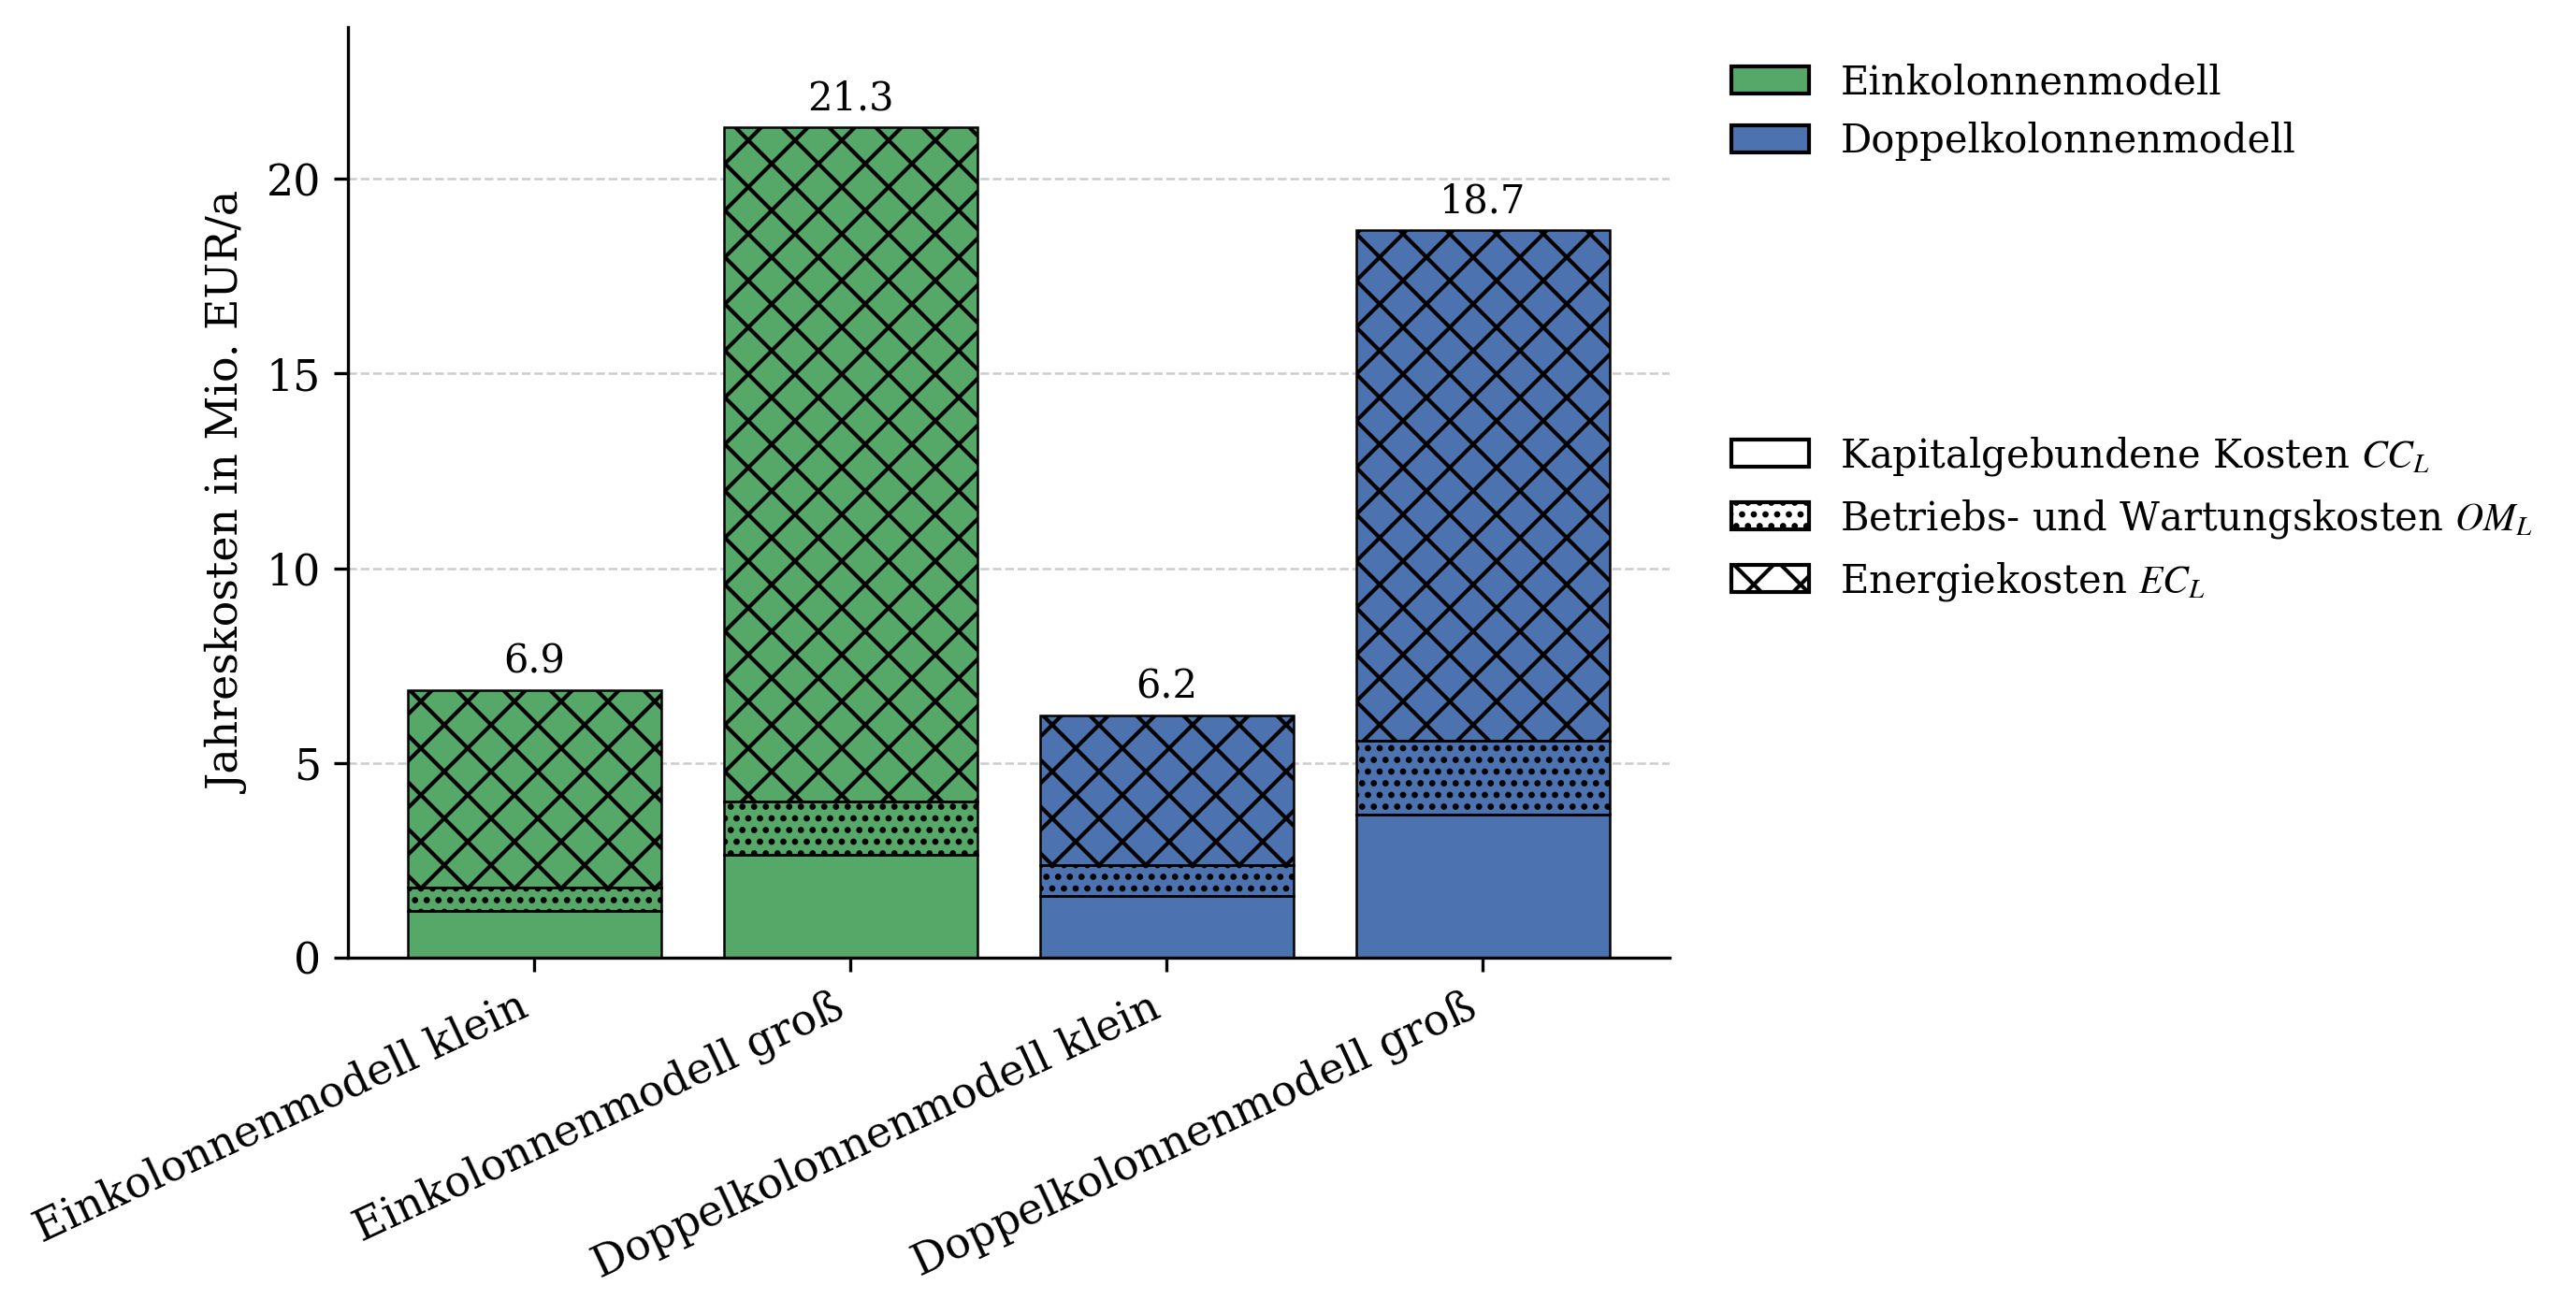
\includegraphics[width=0.90\textwidth]{Overleaf_LaTeX/bilder/trr_zusammensetzung.png}
\caption{Zusammensetzung des jährlichen Total Revenue Requirement \(TRR_L\) aus kapitalgebundenen Kosten \(CC_L\), Betriebs- und Wartungskosten \(OM_L\) sowie Energiekosten \(EC_L\) für die untersuchten Prozessvarianten.}
\label{fig:trr_zusammensetzung}
\end{figure}
\noindent
Die spezifischen Stickstoffbereitstellungskosten \(c_{N_2}\) ergeben sich aus dem Verhältnis der jährlichen Gesamtkosten zur jährlich produzierten Stickstoffmenge. Dadurch können die Varianten unabhängig von ihrer absoluten Anlagengröße miteinander verglichen werden. Während die absoluten Jahreskosten mit der Anlagengröße steigen, verändern sich die spezifischen Kosten nicht im
gleichen Maß, da gleichzeitig eine größere Produktmenge erzeugt wird. Für das Einkolonnenmodell sinken die spezifischen Kosten in der großen Variante leicht, dies ist auch beim Doppelkolonnenmodell zu beobachten. Die niedrigsten spezifischen Stickstoffbereitstellungskosten ergeben sich im
Basisfall für das große Doppelkolonnenmodell mit
\(40{,}78\,\mathrm{EUR\,t_{N_2}^{-1}}\), während die höchsten spezifischen Kosten für das kleine Einkolonnenmodell mit
\(51{,}24\,\mathrm{EUR\,t_{N_2}^{-1}}\) auftreten.
\begin{figure}[H]
\centering
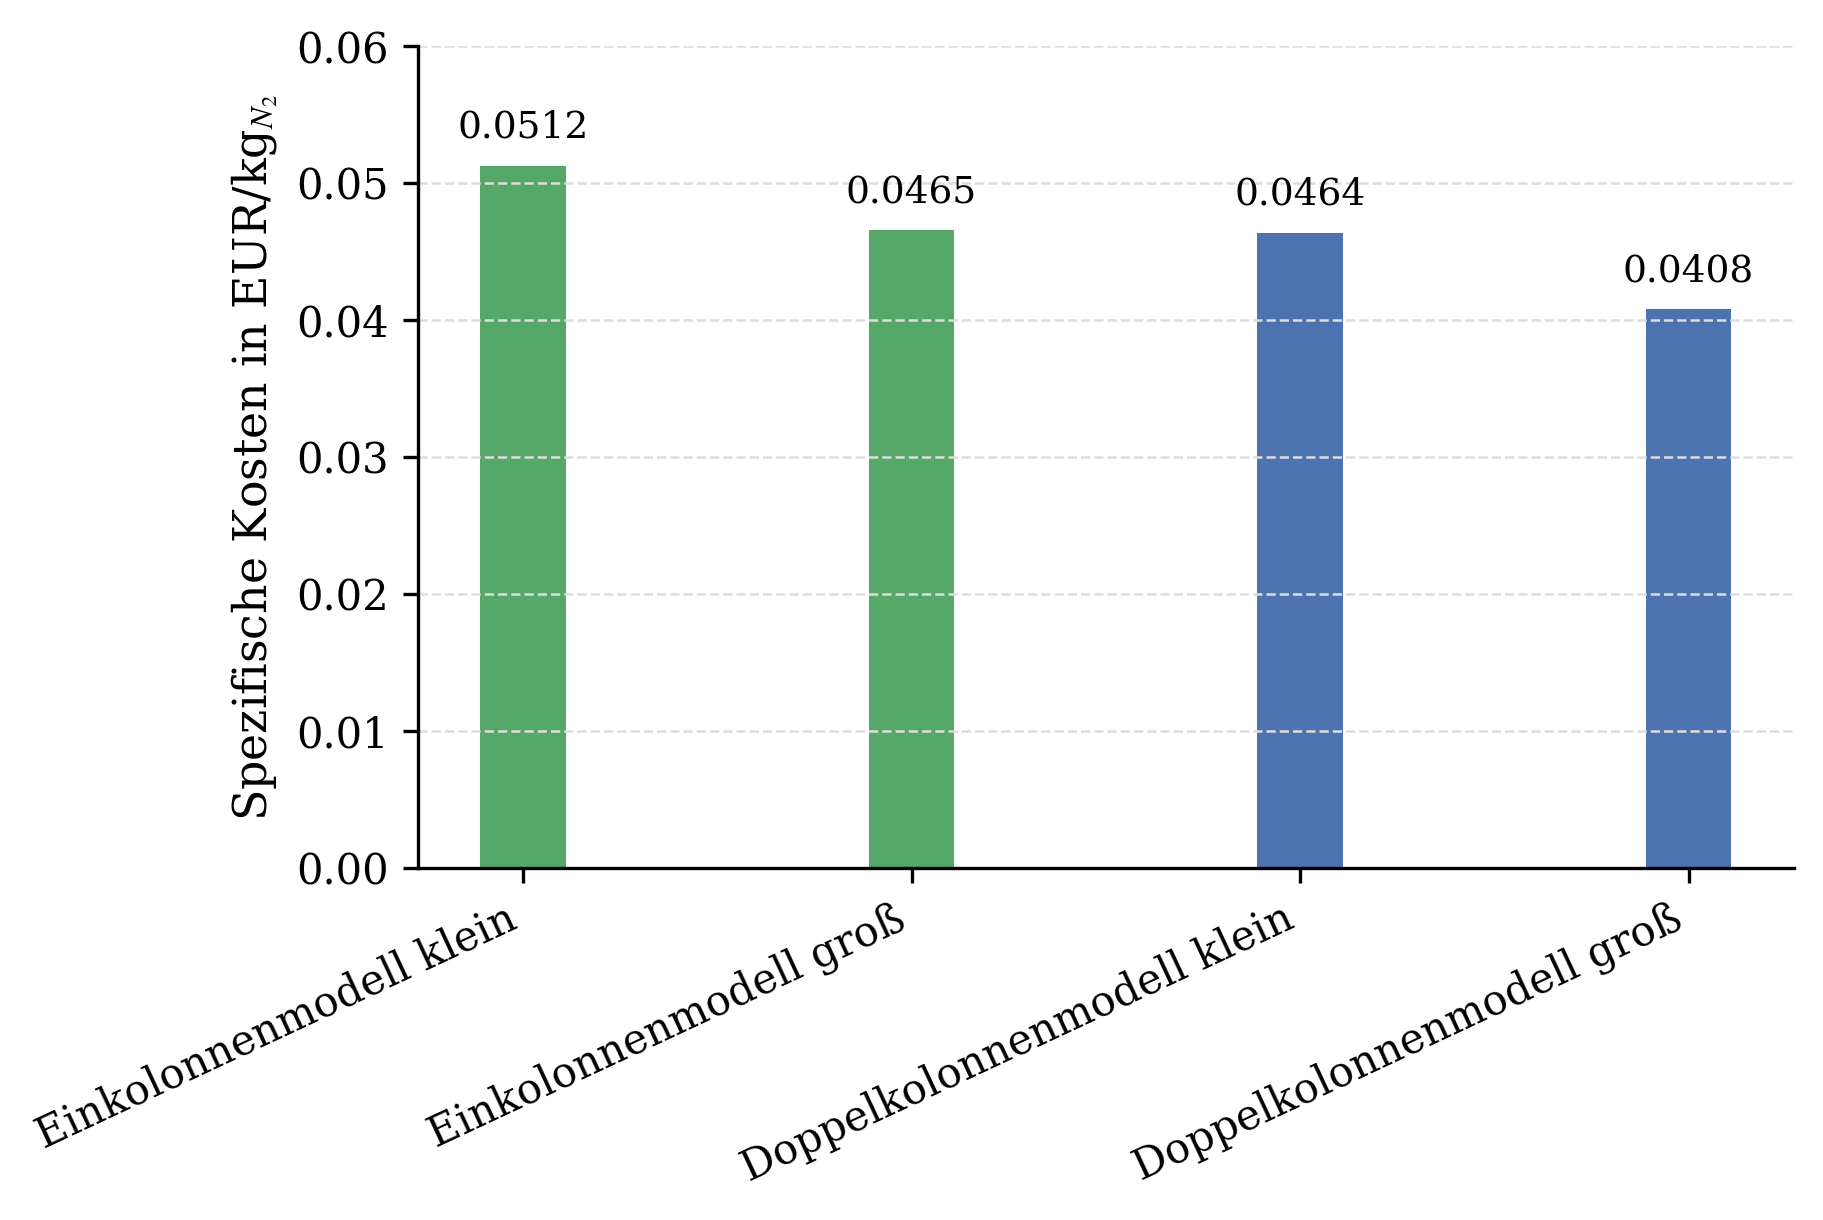
\includegraphics[width=0.75\textwidth]{Overleaf_LaTeX/bilder/spezifische_stickstoffkosten_basisfall.png}
\caption{Spezifische Stickstoffbereitstellungskosten der Einzel- und Doppelkolonnenmodelle im Basisfall. Die Kosten sind auf die erzeugte Stickstoffmasse bezogen und in EUR/kg$_{N_2}$ angegeben.}
\label{fig:spezifische_stickstoffkosten_basisfall}
\end{figure}
\noindent
Die Sensitivität der spezifischen Stickstoffbereitstellungskosten gegenüber dem Strompreis ist in Abbildung  \ref{fig:sensitivitaet_stickstoffkosten_strompreis} dargestellt.
Dazu werden drei Strompreisniveaus von \(\SI{0.13}{\EUR\per\kWh}\),
\(\SI{0.16}{\EUR\per\kWh}\) und \(\SI{0.19}{\EUR\per\kWh}\) betrachtet \cite{SMARDEntwicklungIndustriestrompreise, bdewBDEWStrompreisanalyseApril2026}.\\
In allen Varianten steigen die spezifischen Kosten mit zunehmendem Strompreis annähernd linear an. Dies ist auf den direkten Zusammenhang zwischen Strompreis, elektrischem Netto-Strombedarf und Energiekosten \(EC_L\) zurückzuführen. Der Anstieg fällt beim Einkolonnenmodell stärker aus als beim
Doppelkolonnenmodell. Dies zeigt sich an der steileren Steigung der beiden grünen Verläufe in Abbildung \ref{fig:sensitivitaet_stickstoffkosten_strompreis}. Entsprechend
reagieren die spezifischen Stickstoffbereitstellungskosten des
Einkolonnenmodells im betrachteten Strompreisbereich stärker auf Änderungen des Strompreises.\\
Innerhalb des betrachteten Strompreisbereichs bleibt die relative Reihenfolge der Varianten weitgehend erhalten. Das kleine Doppelkolonnenmodell weist über den gesamten Bereich die niedrigsten spezifischen Kosten auf. Jedoch zeigt das große
Einkolonnenmodell Werte unterhalb des kleinen Doppelkolonnenmodells bei niedrigen Strompreisen.
\begin{figure}[H]
\centering
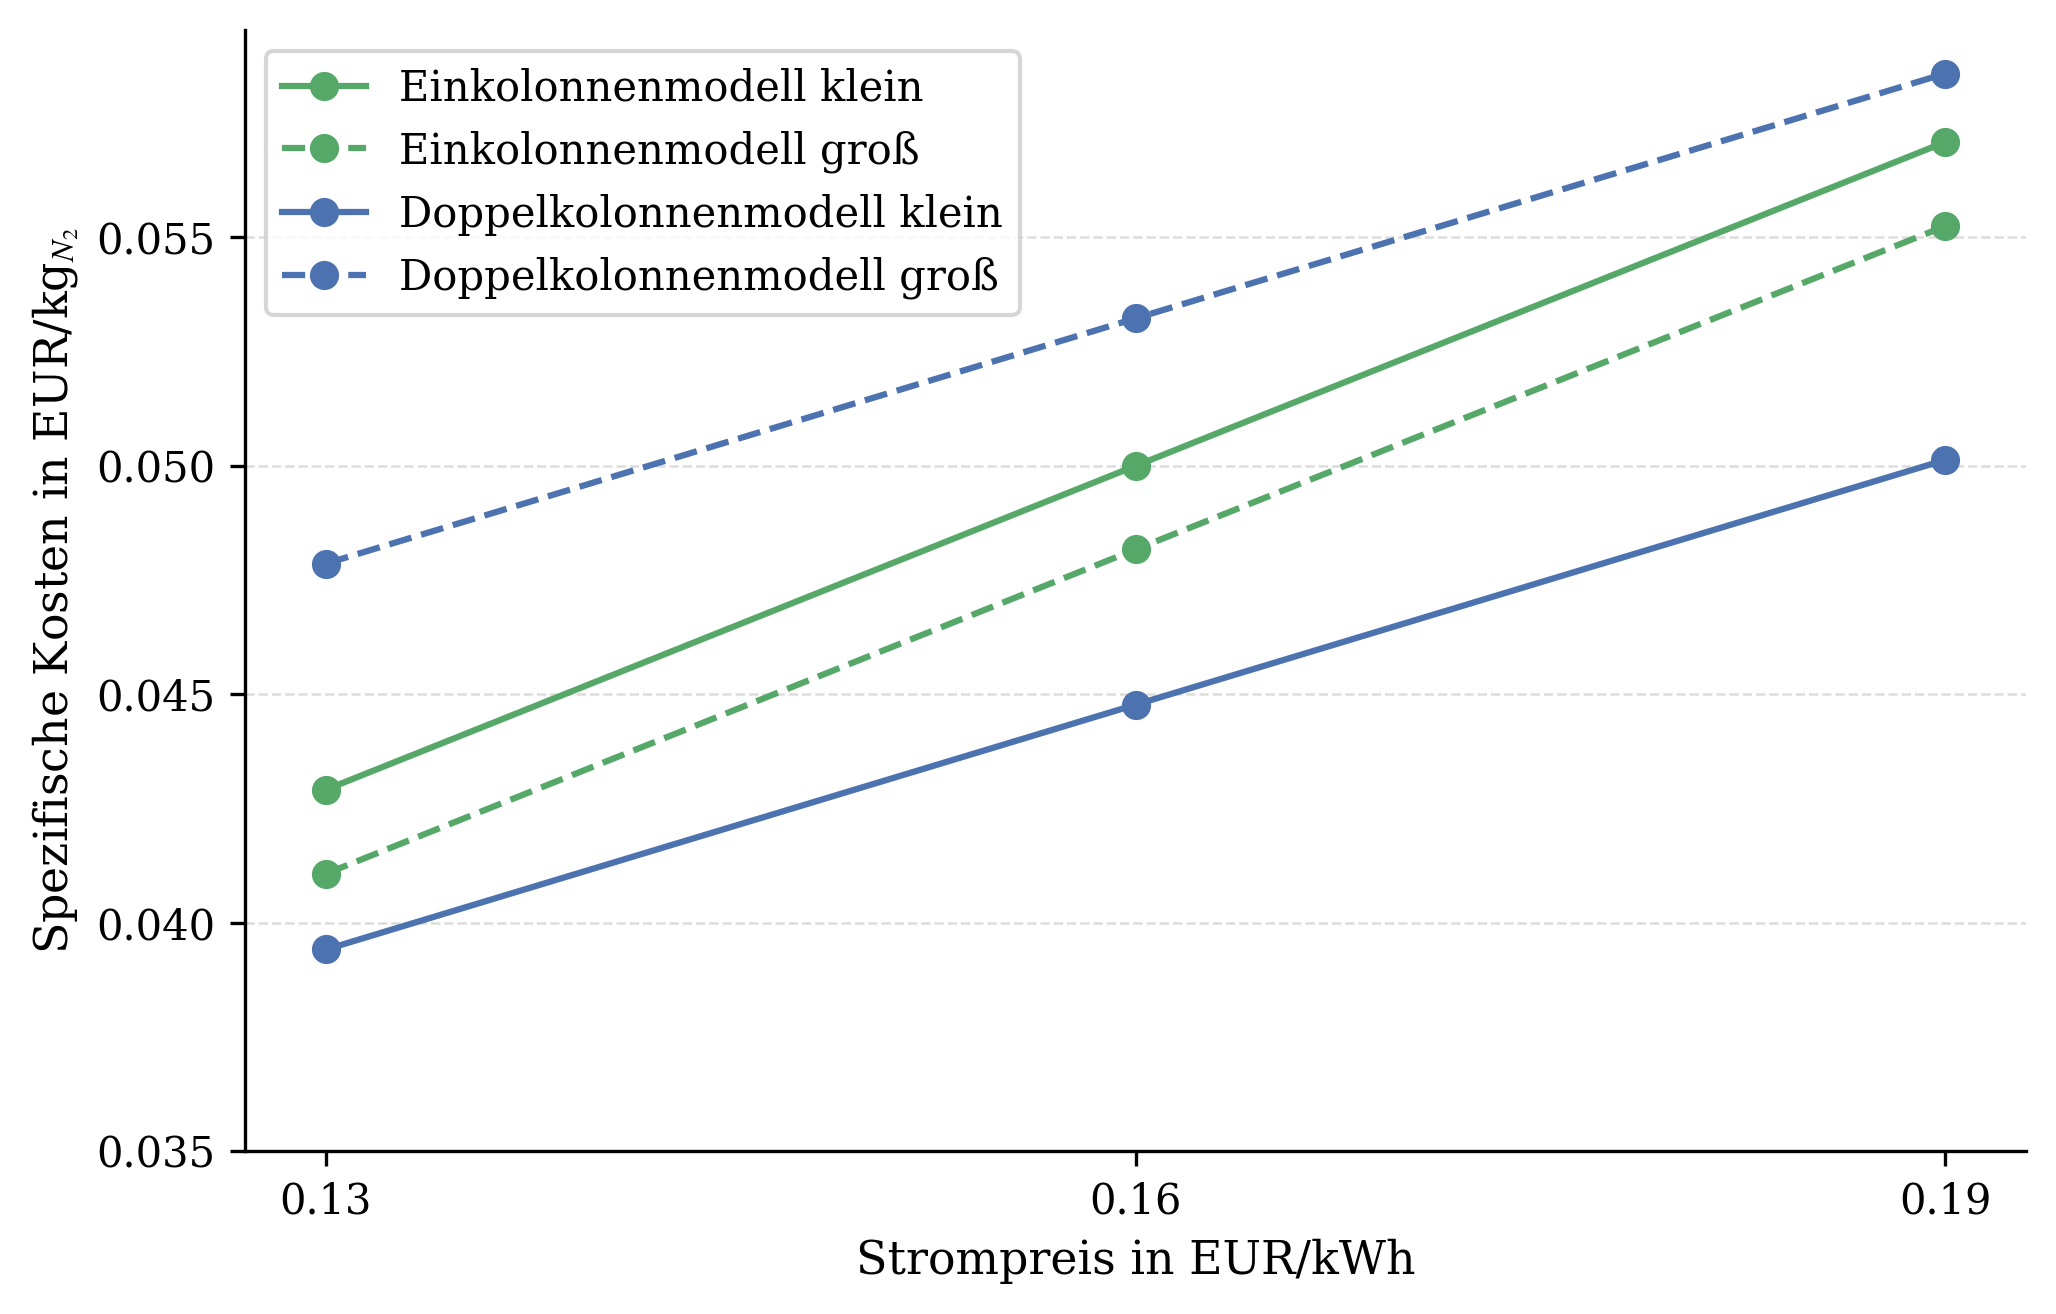
\includegraphics[width=0.80\textwidth]{Overleaf_LaTeX/bilder/sensitivitaet_stickstoffkosten_strompreis.png}
\caption{Sensitivität der spezifischen Stickstoffbereitstellungskosten gegenüber dem angesetzten Strompreis. Dargestellt sind die spezifischen Kosten für Strompreise von \(0{,}13\), \(0{,}16\) und \(0{,}19~\mathrm{EUR/kWh}\).}
\label{fig:sensitivitaet_stickstoffkosten_strompreis}
\end{figure}
\noindent
Abbildung~\ref{fig:sensitivitaet_stickstoffkosten_zinssatz} zeigt, dass die spezifischen
Stickstoffbereitstellungskosten mit steigendem Zinssatz für alle Varianten
zunehmen. Ursache hierfür ist der höhere Anteil der kapitalgebundenen Kosten am
jährlichen Total Revenue Requirement. Der Einfluss des Zinssatzes fällt jedoch
geringer aus als der Einfluss des Strompreises, da die Energiekosten weiterhin
den dominierenden Kostenanteil darstellen.\\
Varianten mit höherem Investitionsaufwand reagieren stärker auf die Änderung
des Zinssatzes. Dies zeigt sich insbesondere beim großen Doppelkolonnenmodell.
Die grundsätzliche Rangfolge der Varianten bleibt im betrachteten Bereich von
\(8\) bis \(12\,\%\) jedoch erhalten.

\begin{figure}[H]
\centering
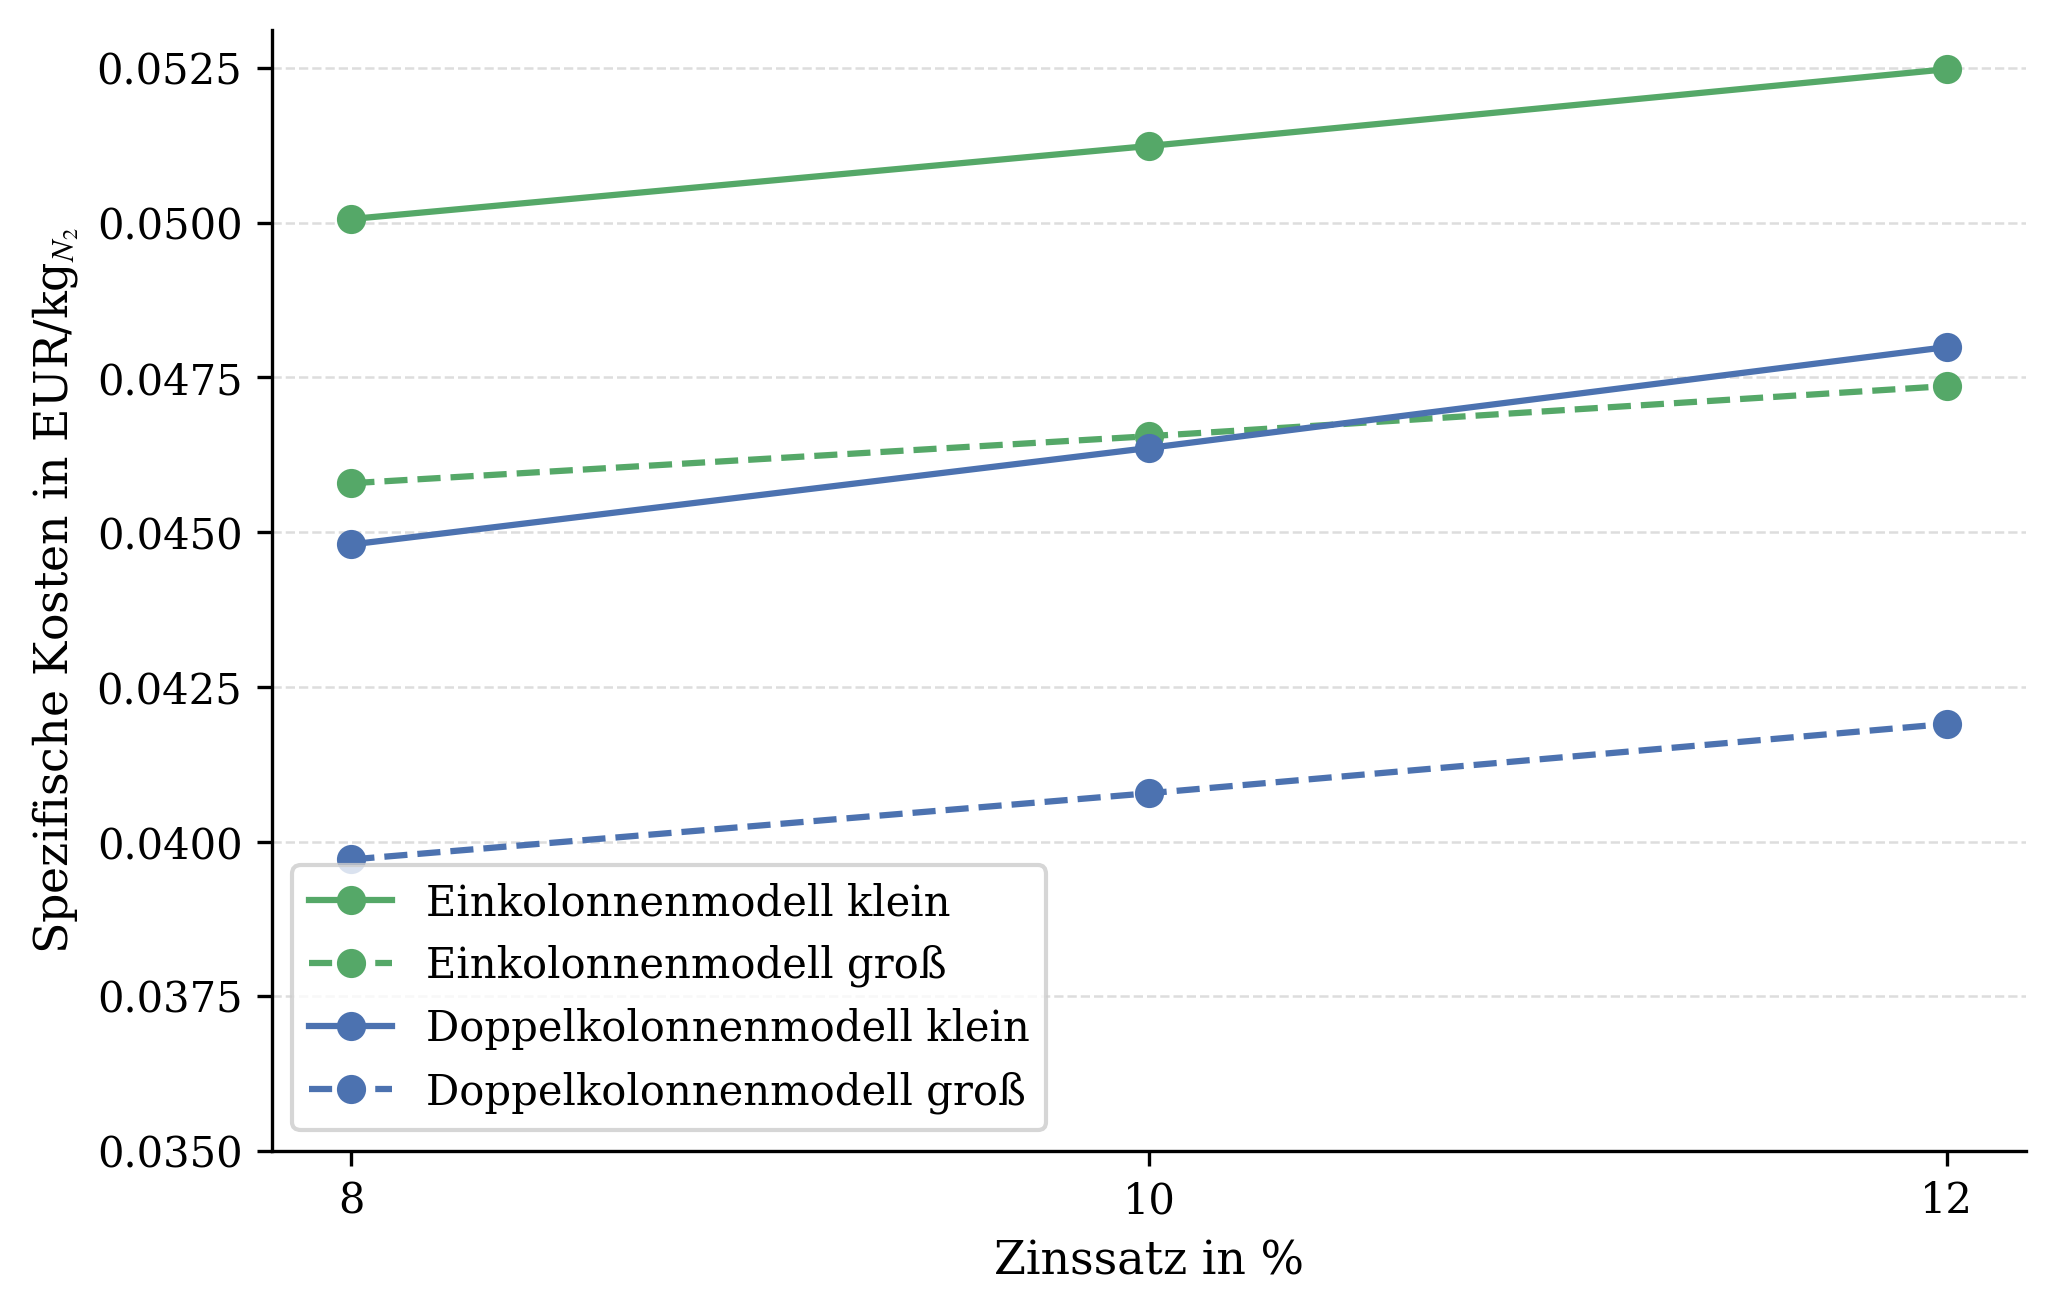
\includegraphics[width=0.80\textwidth]{Overleaf_LaTeX/bilder/sensitivitaet_stickstoffkosten_zins.png}
\caption{Sensitivität der spezifischen Stickstoffbereitstellungskosten gegenüber dem angesetzten effektivem Zinssatz. Dargestellt sind die spezifischen Kosten für einen Zinssaz von \(8\), \(10\) und \(12~\)\%.}
\label{fig:sensitivitaet_stickstoffkosten_zinssatz}
\end{figure}